\documentclass[dvips]{article}
\usepackage{graphics}
\usepackage{subfig}
\setlength{\topmargin}{0mm}
\setlength{\textheight}{220mm}
\setlength{\oddsidemargin}{0mm}
\setlength{\textwidth}{160mm}

\begin{document}
\vspace{40mm}
\begin{center}
{\Large Initial Conditions for Direct Numerical Simulation of
Turbulence}\\[10mm]
R.S.Cant\\
CFD Laboratory\\
Cambridge University Engineering Department\\[30mm]
Report number CUED--THERMO--2012/03\\
August 2012
\end{center}

\newpage
\section{Introduction}
In the Direct Numerical Simulation (DNS) of turbulent flow it is desirable
to specify initial conditions that are already a good approximation to a
turbulent solution of the Navier--Stokes equations.  This ensures that the
simulation will begin to generate a truly turbulent solution as quickly as
possible and without excessive initial transients.
It is also convenient to make use of the initial conditions to set the
values of key turbulence parameters {\it a proiri}.  In the absence
of a Navier--Stokes solution in closed form, or of sufficiently--detailed
experimental data, it is necessary to construct the initial approximation
numerically.  The output
from a previous simulation may be used if the physical and computational
parameters are compatible but it is more often the case that an entirely
new set of turbulent initial conditions is required, for example
where the computational domain size is to be changed or a new statistical
realisation of the turbulence is needed.  This report
gives a detailed account of a method for producing an excellent numerical 
approximation to a field of three--dimensional homogeneous isotropic turbulence
having a specified energy spectrum and satisfying the continuity constraint
for incompressible flow.  The method was suggested by Orszag \cite{orszaginit}
in the context of DNS using spectral methods and was refined by Rogallo
\cite{rogallo} and by Lee and Reynolds \cite{leereynolds}.
Subsequently it has become a standard procedure for generating turbulent
initial conditions for DNS, and this report describes its implementation
in both serial and parallel codes for DNS of turbulent combustion.

It is worth noting that the restriction to incompressible flow allows for
significant simplifications in both the mathematical formulation and the
computational implementation
of the turbulent initial velocity field.  
In practice this does not preclude the use of such an
initial field to start a compressible or reacting flow simulation,
provided that the subsequent evolution of the additional physics
is well described.

Thus the aim is to generate a field of incompressible homogeneous isotropic
turbulence having a specified energy spectrum function $E(\bar{k})$,
where $\bar{k}$ is the wavenumber vector magnitude
in the Fourier--space representation of the turbulent velocity field.
Note that $\bar{k}$ is defined as a {\it linear} wavenumber or inverse
wavelength, as distinct from an {\it angular} wavenumber with vector
magnitude $\hat{k}=2\pi \bar{k}$
which is used extensively in the classical literature.
The function $E(\bar{k})$ is central to the procedure, since it defines
among other things the initial value of the turbulence RMS
fluctuation magnitude $u$, the turbulence integral length scale $L$,
the Taylor length scale $\lambda$ and the Kolmogorov length scale $\eta$,
as well as the turbulence energy dissipation rate $\varepsilon$.

The remainder of the report contains a brief account of the underlying theory
as presented in detail by Batchelor \cite{batchelor53}, together with a
discussion of the properties of the spectrum function and its
relationship to the principal properties of the turbulence.  This is followed
by a description of the computational implementation of the method for
generating turbulent initial conditions.

\section{Theoretical Development}
The intention is to ensure that the initial turbulent velocity field
satisfies the conditions for continuity, homogeneity and isotropy.  From the
theoretical standpoint it is most convenient to do this in Fourier
space.

\subsection{Continuity}
For incompressible flow the continuity condition is
\begin{equation}
\nabla . \underline{u} = 0
\label{CONTPHYS}
\end{equation}
which may be expressed in Fourier space as
\begin{equation}
\underline{\bar{k}}.\underline{\hat{u}}(\underline{k}) = 0
\label{CONTFOUR}
\end{equation}
where $\underline{\hat{u}}(\underline{\bar{k}})$ is the Fourier transform of the
real--space velocity vector $\underline{u}(\underline{x})$:
\begin{eqnarray}
\underline{\hat{u}}(\underline{\bar{k}}) & = & \int \underline{u}(\underline{x})
\exp{(i2\pi\underline{\bar{k}}.\underline{x})} d\underline{x}
\label{FOURTRAN}\\
\underline{u}(\underline{x}) & = & \int
\underline{\hat{u}}(\underline{\bar{k}})
\exp{(-i2\pi\underline{\bar{k}}.\underline{x})} d\underline{\bar{k}}
\label{FOURINV}
\end{eqnarray}
Note that the Fourier transform is defined here using standard modern
practice, and that this differs in matters of detail from the
older definition used by Batchelor \cite{batchelor53}.
In order for the integrals in (\ref{FOURTRAN}) and (\ref{FOURINV})
to exist it is necessary for the real--space velocity $\underline{u}$
to satisfy certain criteria \cite{batchelor53}, and in practice it is
sufficient as
well as simple and elegant to assume that $\underline{u}$ is
periodic in all three directions.

\subsection{Homogeneity}
An important quantity to consider is the velocity correlation
tensor $R_{ij}(\underline{r})$ defined as
\begin{equation} 
R_{ij}(r) = \overline{u_{i}(\underline{x})u_{j}(\underline{x}+\underline{r})}
\end{equation} 
where the overbar indicates a time, space or ensemble average over the
probability distribution of the velocity.  The condition
of homogeneity is assured by noting that $R_{ij}$ is a function of the
spacing vector $\underline{r}$ only and does not depend on the position vector
$\underline{x}$.  As the spacing $\underline{r}$ tends to zero the
velocity correlation tensor reduces to the Reynolds stress tensor
\begin{equation} 
r_{ij} = R_{ij}(0) = \overline{u_{i}(\underline{x})u_{j}(\underline{x})}
\end{equation} 
which is independent of spatial position due to the assumption of homogeneity.
The trace of the Reynolds stress tensor is equal to twice the turbulent kinetic
energy per unit mass, ie
\begin{equation}
K = \frac{1}{2}r_{ii}
= \frac{1}{2}\overline{u_{i}(\underline{x})u_{i}(\underline{x})}
\end{equation}
The Fourier transform of $R_{ij}$ is the energy
spectrum tensor $\Phi_{ij}$ defined as
\begin{equation}
\Phi_{ij}(\underline{\bar{k}}) = \int R_{ij}(\underline{r})
\exp{(i2\pi\underline{\bar{k}}.\underline{r})} d\underline{r}
\label{SPECTENS}
\end{equation}
and the physical meaning of this tensor can be made clear by considering the
inverse transform
\begin{equation}
R_{ij}(\underline{r}) = \int \Phi_{ij}(\underline{\bar{k}})
\exp{(-i2\pi\underline{\bar{k}}.\underline{r})} d\underline{\bar{k}}
\label{SPECTENSINV}
\end{equation}
Setting the spacing vector $\underline{r}$ to zero in this expression yields
\begin{equation}
R_{ij}(0) = r_{ij} = \int \Phi_{ij}(\underline{\bar{k}})
d\underline{\bar{k}}
\end{equation}
so that $\Phi_{ij}$ is shown to describe the contribution to the
correlation tensor $R_{ij}$
arising from each element of wavenumber in Fourier space.  In particular,
it follows that half of the trace $\Phi_{ii}$ of the energy spectrum
tensor represents the energy density of the turbulence in Fourier space:
\begin{equation}
K = \frac{1}{2}r_{ii} = \int \frac{1}{2}\Phi_{ii}(\underline{\bar{k}})
d\underline{\bar{k}}
\label{TKE}
\end{equation}
 
A slightly different perspective is obtained by averaging $\Phi_{ij}$
over all directions in Fourier space according to
\begin{equation}
\Psi_{ij}(k) = \int \Phi_{ij}(\underline{\bar{k}}) dA(\bar{k})
\label{PSIDEF}
\end{equation}
where $\bar{k} = \sqrt{\bar{k}_{i}\bar{k}_{i}}$ is the wavenumber vector
magnitude and $dA(\bar{k})$ denotes an element of the area of a sphere in
Fourier space at
radius $\bar{k}$.  Then the directionally--averaged tensor
$\Psi_{ij}(\bar{k})$ represents
the contribution to the energy spectrum tensor from a small element of
wavenumber magnitude $d\bar{k}$ forming a spherical shell at radius
$\bar{k}$.

In passing, it is useful to note that the one--dimensional spectrum functions
$\Theta_{ij}$ may be obtained by
integrating the energy spectrum tensor over two of the components of the vector
argument $\underline{\bar{k}}$.  Choosing without loss of generality to take
$\bar{k}_{1}$ as the surviving component yields
\begin{equation}
\Theta_{ij}(\bar{k}_{1}) = \int_{-\infty}^{\infty} \int_{-\infty}^{\infty}
\Phi_{ij}(\bar{k}_{1},\bar{k}_{2},\bar{k}_{3})dk_{2}dk_{3}.
\label{SPECF1D}
\end{equation}
The longitudinal one--dimensional spectrum function
$\Theta_{11}(\bar{k}_{1})$ is obtained by setting $i=j=1$,
while the lateral one--dimensional spectrum functions
$\Theta_{22}(\bar{k}_{1})$ or $\Theta_{33}(\bar{k}_{1})$ are obtained by
setting $i=j\neq 1$.\\[2mm]

\subsection{Isotropy}
The condition of isotropy is met by noting that the tensor $\Phi_{ij}$
must have a specific form in isotropic turbulence \cite{batchelor53}:
\begin{equation}
\Phi_{ij}(\underline{\bar{k}}) = F_{k}(\bar{k})\bar{k}_{i}\bar{k}_{j} +
G_{k}(\bar{k})\delta_{ij}
\end{equation}
where $F_{k}$ and $G_{k}$ are functions only of the wavenumber
vector magnitude.  Using the continuity condition (\ref{CONTFOUR}) it may
be shown that
\begin{equation}
\frac{\partial}{\partial r_{i}}R_{ij} =
\frac{\partial}{\partial r_{j}}R_{ij} = 0
\label{CONTVELCOR}
\end{equation}
and from the definition (\ref{SPECTENSINV}) it follows that
\begin{equation}
\bar{k}_{i}\Phi_{ij} =
\bar{k}_{j}\Phi_{ij} = 0.
\label{CONTSPECTENS}
\end{equation}
Then the functions $F_{k}$ and $G_{k}$ are seen to be related according to
$G_{k} = -\bar{k}^{2}F_{k}$, and the tensor $\Phi_{ij}$ 
is specified completely by a single function $F_{k}$ of wavenumber vector
magnitude.  Since the turbulence is isotropic then by definition
there is no preferred direction and the surfaces of constant
energy in Fourier space are spheres.  The energy contained within a
spherical shell of thickness $d\bar{k}$ at a wavenumber magnitude
$\bar{k}$ is defined as $E(\bar{k})d\bar{k}$ where $E(\bar{k})$ is the
energy spectrum function.  According
to this definition together with (\ref{PSIDEF}) the energy spectrum
function is given by
\begin{equation}
E(\bar{k}) = \frac{1}{2}\Psi_{ii}(\bar{k}) =
\frac{1}{2}\Phi_{ii}(\bar{k})\int dA(\bar{k})
\end{equation}
where the second step follows due to isotropy.  Thus 
the energy spectrum function becomes 
\begin{equation}
E(\bar{k}) = 4\pi \bar{k}^{2} \frac{1}{2}\Phi_{ii}(\underline{\bar{k}})
\label{ESPECT}
\end{equation}
and the energy spectrum tensor for homogeneous isotropic turbulence 
is fully defined by
\begin{equation}
\Phi_{ij}(\underline{\bar{k}}) = \frac{E(\bar{k})}{4\pi
\bar{k}^{4}}(\bar{k}^{2}\delta_{ij}-\bar{k}_{i}\bar{k}_{j})
\label{SPECISO}
\end{equation}

In order to obtain expressions for the individual Fourier--space velocity
components $\hat{u}_{i}(\bar{k})$ it is necessary to relate these to the 
spectrum tensor.  Batchelor \cite{batchelor53} notes that the physical--space
velocity is given by
\begin{equation}
\underline{u}(\underline{x}) = \int
\exp{(-i2\pi\underline{\bar{k}}.\underline{x})}
d\underline{Z}(\underline{\bar{k}})
\label{ZVELS}
\end{equation}
where $d\underline{Z}(\underline{\bar{k}})$ is a vector of statistically
independent random increments.  Comparing with the Fourier transform
definition (\ref{FOURINV}) it is clear that in the present case
$d\underline{Z}(\underline{\bar{k}}) =
\underline{\hat{u}}(\underline{\bar{k}})d\underline{\bar{k}}$,
so that the Fourier--space
velocity values $\underline{\hat{u}}(\underline{\bar{k}})$ must
themselves be random in
nature.  Substituting (\ref{ZVELS}) in the definition (\ref{SPECTENS})
of the spectrum tensor it follows that
\begin{equation}
\Phi_{ij}(\underline{\bar{k}})
= \overline{\hat{u}_{i}(-\underline{\bar{k}})\hat{u}_{j}(\underline{\bar{k}})}
\end{equation} 
and since the velocity in physical space is purely real the symmetry condition
\begin{equation}
\hat{u}_{i}(-\underline{\bar{k}})=\hat{u}_{j}^{*}(\underline{\bar{k}})
\label{VELSYM}
\end{equation}
may be applied, where $*$ denotes the complex conjugate, so that
\begin{equation}
\Phi_{ij}(\underline{\bar{k}})
= \overline{\hat{u}_{i}^{*}(\underline{\bar{k}})\hat{u}_{j}(\underline{\bar{k}})}
\label{SPECVELS}
\end{equation} 
Note that this result is different from that obtained using the
correlation theorem in the case where the Fourier--space velocities are
deterministic.  In the present case it is necessary also to average over the
probability space of the random velocity components.  The
implication is that the energy spectrum, as well as the conditions of
homogeneity and isotropy, is accurate only in a statistical sense and that
individual realisations of the velocity field may deviate significantly
from the specified average.

\section{Synthesis of the Initial Velocity Field}
In constructing a realisation of the velocity field it is useful to note
that the continuity equation (\ref{CONTFOUR}) states that
the Fourier--space velocity vector $\underline{\hat{u}}$ is orthogonal
to the wavenumber vector $\underline{\bar{k}}$.  Thus there is no component of
$\underline{\hat{u}}$ in the direction of the wavenumber vector and it
is possible to write an expression for the Fourier--space velocity vector
having only two components:
\begin{equation}
\underline{\hat{u}}(\underline{\bar{k}}) = \alpha(\underline{\bar{k}})\underline{e}_{1}
+ \beta(\underline{\bar{k}})\underline{e}_{2}
\label{VELFAB}
\end{equation}
Here, the system of unit basis vectors $\underline{e}_{1}$,
$\underline{e}_{2}$ and $\underline{e}_{3}$ is defined
such that $\underline{e}_{3}$ is aligned with $\underline{\bar{k}}$, and the
complex functions $\alpha$ and $\beta$ are yet to be defined.
In this coordinate system the trace of the spectrum tensor may be expressed
using (\ref{SPECVELS}) and (\ref{VELFAB}) as
\begin{equation}
\Phi_{ii}(\underline{\bar{k}}) = \frac{E(\bar{k})}{2\pi \bar{k}^{2}}
 = \overline{\alpha\alpha^{*} + \beta\beta^{*}}
\label{SPECBAR}
\end{equation}

In DNS it is possible to resolve only a limited range of scales, and a
consequence is that the large scales of motion, while always well resolved,
may be poorly sampled.  In the present case the surfaces of constant energy
in Fourier space are spheres, but the DNS computational grid 
corresponds in Fourier space to a regular cubic grid of points, each of
which supports a single Fourier mode.  The number of modes available
to represent the motion up to a given energy level corresponds to the number
of points contained within the sphere.  For low wavenumbers the radius
of the sphere is small and the number of modes is strictly limited.
Physically this corresponds to the simple fact
that only a small number of large eddies may be fitted into
the computational box.  Statistically the resulting small sample of large
eddies may not be truly representative, and it is rarely possible to repeat
the simulation many times in order to check the average expressed by
the overbar in (\ref{SPECVELS}).
A straightforward method which avoids this issue is
to strengthen the condition implied by (\ref{SPECBAR}) and to insist
that each Fourier mode
must conform separately to the average energy:
\begin{equation}
\Phi_{ii}(\underline{\bar{k}}) = \frac{E(\bar{k})}{2\pi \bar{k}^{2}}
 = \alpha\alpha^{*} + \beta\beta^{*}
\label{KCOND}
\end{equation}
The simplest expressions for $\alpha$ and $\beta$ which satisfy
this constraint are 
\begin{eqnarray}
\alpha & = & \sqrt{\frac{E(\bar{k})}{2\pi \bar{k}^{2}}}e^{i\theta_{1}}\cos{\phi}\nonumber\\
\beta & = & \sqrt{\frac{E(\bar{k})}{2\pi \bar{k}^{2}}}e^{i\theta_{2}}\sin{\phi}
\label{ALPHABET}
\end{eqnarray}
where $\theta_{1}$ and $\theta_{2}$ are phase angles defined on the
interval $[-\pi,\pi)$, and $\phi$ is the azimuthal angle defined on the
interval $[0,2\pi)$ that specifies the angular position
of the $\underline{e}_{1}$ vector in the plane normal
to the wavenumber vector $\underline{\bar{k}}$.  In order to provide the
degree of randomness required according to (\ref{ZVELS}), all three angles
are treated as uniformly--distributed random numbers with probability
density functions
\begin{eqnarray}
P_{\theta}(\theta_{1}) & = & \frac{1}{2\pi},\hspace{2mm}-\pi\le\theta_{1} < \pi;
\hspace{2mm} 0 \hspace{1.5mm}{\rm otherwise} \\
P_{\theta}(\theta_{2}) & = & \frac{1}{2\pi},\hspace{2mm}-\pi\le\theta_{2} < \pi;
\hspace{2mm} 0 \hspace{1.5mm}{\rm otherwise} \\
P_{\phi}(\phi) & = & \frac{1}{2\pi},\hspace{2mm}0\le\phi < 2\pi;
\hspace{2mm} 0 \hspace{1.5mm}{\rm otherwise}
\end{eqnarray}

Having calculated the components of the Fourier--space velocity vector in
the special coordinate system that has $\underline{e}_{3}$ aligned with
$\underline{k}$ it is necessary to determine a rotation of axes that will
provide the velocity components in the original coordinate system that
defines the computational grid.  The computational basis vectors are 
given by $\underline{b}_{1}=(1,0,0)$, $\underline{b}_{2}=(0,1,0)$,
$\underline{b}_{3}=(0,0,1)$, and in this coordinate system the
$\underline{k}$-aligned basis vectors have components
\begin{eqnarray}
\underline{e}_{1} & = & \left(e_{11},e_{12},e_{13}\right) \nonumber\\
\underline{e}_{2} & = & \left(e_{21},e_{22},e_{23}\right) \nonumber\\
\underline{e}_{3} & = &
\left(\frac{\bar{k}_{1}}{\bar{k}},\frac{\bar{k}_{2}}{\bar{k}},\frac{\bar{k}_{3}}{\bar{k}}\right)  
\end{eqnarray}
where the $e_{ij}$ are to be determined.  Since the azimuthal angle
$\phi$ is random there is freedom to choose the orientation of the
$\underline{e}_{1}$ vector in the plane normal to
$\underline{e}_{3}=\underline{\bar{k}}$.  It is convenient to fix
$\underline{e}_{1}$ to lie within the $\underline{b}_{1}-\underline{b}_{2}$
plane and this is achieved by setting $e_{13}=0$.  Then the remaining
components follow from the orthogonality and normalisation conditions on
the basis vectors to yield
\begin{eqnarray}
\underline{e}_{1} & = &
\left(\frac{\bar{k}_{2}}{M},-\frac{\bar{k}_{1}}{M},0\right) \nonumber\\
\underline{e}_{2} & = &
\left(\frac{\bar{k}_{1}\bar{k}_{3}}{\bar{k}M},\frac{\bar{k}_{2}\bar{k}_{3}}{\bar{k}M},
-\frac{\bar{k}_{1}^{2}+\bar{k}_{2}^{2}}{\bar{k}M}\right) \nonumber\\
\underline{e}_{3} & = &
\left(\frac{\bar{k}_{1}}{\bar{k}},\frac{\bar{k}_{2}}{\bar{k}},\frac{\bar{k}_{3}}{\bar{k}}\right)  
\end{eqnarray}
where $M=\sqrt{\bar{k}_{1}^{2}+\bar{k}_{2}^{2}}$.  The rotation matrix required to transform
a vector from the $\underline{\bar{k}}$-aligned basis into the computational
basis is
\begin{equation}
\underline{b}_{(i)}.\underline{e}_{(j)} = 
\left(
\begin{array}{ccc}
\frac{\bar{k}_{2}}{M}   &  \frac{\bar{k}_{1}\bar{k}_{3}}{\bar{k}M}
&  \frac{\bar{k}_{1}}{\bar{k}} \\[2mm]
-\frac{\bar{k}_{1}}{M}  &  \frac{\bar{k}_{2}\bar{k}_{3}}{M}            &
\frac{\bar{k}_{2}}{\bar{k}} \\[2mm]
0                 &  -\frac{\bar{k}_{1}^{2}+\bar{k}_{2}^{2}}{M}  &
\frac{\bar{k}_{3}}{M} 
\end{array}
\right)
\end{equation}
and this may be applied to the Fourier--space velocity vector (\ref{VELFAB})
to yield
\begin{eqnarray}
\hat{u}_{1}(\underline{\bar{k}}) & = &
\frac{\alpha \bar{k} \bar{k}_{2} + \beta \bar{k}_{1}
\bar{k}_{3}}{\bar{k}M} \nonumber \\
\hat{u}_{2}(\underline{\bar{k}}) & = &
\frac{\beta \bar{k}_{2} \bar{k}_{3} - \alpha \bar{k}
\bar{k}_{1}}{\bar{k}M} \nonumber \\
\hat{u}_{3}(\underline{\bar{k}}) & = &
-\frac{\beta (\bar{k}_{1}^{2}+\bar{k}_{2}^{2})}{\bar{k}M}
\label{VELFOUR}
\end{eqnarray}

\subsection{Verification}
It is simple to verify that the prescription given above exactly satisfies
both the continuity condition (\ref{CONTFOUR}) and the strengthened
energy condition (\ref{KCOND}).  Thus the single realisation of the
turbulent velocity field specified by
(\ref{VELFOUR}) is divergence--free and conforms to the required energy
spectrum function $E(\bar{k})$ in a deterministic manner.  Substituting
(\ref{VELFOUR}) in the expression (\ref{SPECVELS}) for the spectrum tensor  
$\Phi_{ij}(\underline{\bar{k}})$ it is possible to recover the
expression (\ref{SPECISO}) for the spectrum tensor in isotropic turbulence,
but it is interesting to note that the condition for isotropy is satisfied only 
in the mean.  For example, the component $\Phi_{11}$ is given by
\begin{eqnarray}
\Phi_{11} & = & \overline{\hat{u}_{1}^{*}\hat{u}_{1}} \nonumber \\
& = & \frac{1}{\bar{k}^{2}M^{2}}\left[
\overline{\alpha^{*}\alpha}\bar{k}^{2}\bar{k}_{2}^{2}
+(\overline{\alpha^{*}\beta}+\overline{\beta^{*}\alpha})\bar{k}\bar{k}_{1}\bar{k}_{2}\bar{k}_{3}
+\overline{\beta^{*}\beta}\bar{k}_{1}^{2}\bar{k}_{3}^{2}
\right]
\end{eqnarray}
The averages denoted by the overbars on the terms in $\alpha$ and $\beta$
may be evaluated by substituting for
$\alpha$ and $\beta$ from (\ref{ALPHABET}) and integrating over the 
probability density function for each of the angles $\theta_{1}$, $\theta_{2}$ and $\phi$:
\begin{eqnarray}
\overline{\alpha^{*}\alpha} & = &
\frac{E(\bar{k})}{2\pi \bar{k}^{2}}\overline{\cos^{2}{\phi}} =
\frac{E(\bar{k})}{4\pi \bar{k}^{2}} \nonumber\\
\overline{\alpha^{*}\beta} & = &
\frac{E(\bar{k})}{2\pi
\bar{k}^{2}}\overline{e^{i(\theta_{2}-\theta_{1})}\cos{\phi}\sin{\phi}}
= 0 \nonumber\\
\overline{\beta^{*}\alpha} & = &
\frac{E(\bar{k})}{2\pi
\bar{k}^{2}}\overline{e^{i(\theta_{1}-\theta_{2})}\cos{\phi}\sin{\phi}}
= 0 \nonumber\\
\overline{\beta^{*}\beta} & = &
\frac{E(\bar{k})}{2\pi \bar{k}^{2}}\overline{\sin^{2}{\phi}} = \frac{E(\bar{k})}{4\pi \bar{k}^{2}}
\end{eqnarray}
Thus the spectrum tensor component $\Phi_{11}$ becomes
\[
\Phi_{11} = \frac{E(\bar{k})}{4\pi \bar{k}^{2}}(\bar{k}^{2}-\bar{k}_{1}^{2})
\]
as required, and all of the remaining components follow in a similar manner.
It is important to note that the averaging operation here is carried out
notionally over
an ensemble of many realisations of the turbulent velocity field, and that
any single realisation may deviate significantly from isotropy due to the
small sample of low--wavenumber modes.

It should also be noted that the prescription (\ref{VELFOUR}) does not
automatically recover
the symmetry condition expressed by (\ref{VELSYM}), which must be imposed
explicitly in order to ensure that the initial velocity field in physical
space takes values that are purely real.

\subsection{Limiting cases}
In generating a velocity field using (\ref{VELFOUR}) some care
is required when the denominator of each expression is equal to zero.  This can
occur when either $\bar{k}=0$, or when $M=0$ with $\bar{k}_{3}$ fixed and
non--zero.
When $\bar{k}=0$ it is expected that the spectrum function $E(0)$ is
identically zero.  Given suitable limiting
behaviour of $E(\bar{k})$ as $\bar{k}\rightarrow 0$, both $\alpha$ and $\beta$
are identically zero in the limit and no difficulty arises since all
components $(\hat{u}_{1},\hat{u}_{2},\hat{u}_{3})$ vanish.
It is interesting to note that the manner in which 
$E(\bar{k}) \rightarrow 0$ as $\bar{k} \rightarrow 0$ has far--reaching
theoretical consequences (see, for example, \cite{moninyag}).

By contrast, the case $M\rightarrow 0$, $\bar{k}_{3}\neq 0$ in general has
$E(\bar{k})\neq 0$ and
special consideration is required in the evaluation of the velocity components
in order to produce the correct value of the turbulent kinetic energy.  Since
$\bar{k}^{2} = M^{2}+\bar{k}_{3}^{2}$, then as $M$ becomes much smaller
than $\bar{k}_{3}$
it is clear that $\bar{k}\simeq \bar{k}_{3}$.  Also, it is helpful to
express $\bar{k}_{1} = M\cos\psi$ and $\bar{k}_{2} = M\sin\psi$ where
$\psi$ is an angle in the $\bar{k}_{1}$--$\bar{k}_{2}$ plane.
According to (\ref{VELFOUR}) the velocity components become
\begin{eqnarray}
\hat{u}_{1}(\underline{\bar{k}}) & \simeq &
\frac{\alpha \bar{k}_{2}}{M}
+ \frac{\beta \bar{k}_{1}}{M}
= \alpha\sin\psi+\beta\cos\psi \nonumber \\
\hat{u}_{2}(\underline{\bar{k}}) & \simeq &
\frac{\beta \bar{k}_{2}}{M}
- \frac{\alpha \bar{k}_{1}}{M}
= \beta\sin\psi-\alpha\cos\psi \nonumber \\
\hat{u}_{3}(\underline{\bar{k}}) & = & 0
\end{eqnarray}
The angle $\psi$ is arbitrary, since the azimuthal angle $\phi$ (see
eq.\ref{ALPHABET}) has already been chosen at random and the energy condition
(\ref{KCOND}) is satisfied automatically.  Taking $\psi = \pi/2$ makes
$\bar{k}_{1}=0$ and $\bar{k}_{2} = M$, giving velocity components
$\hat{u}_{1}=\alpha$ and $\hat{u}_{2}=\beta$.
The randomness inherent in the definitions of $\alpha$ and $\beta$ remains
unaffected, and the continuity and isotropy conditions are satisfied.

\section{The Energy Spectrum Function}
The energy spectrum function $E(\bar{k})$ plays a crucial role in defining the
initial turbulence.  It describes the distribution of turbulence kinetic
energy in each
spherical shell of Fourier space characterised by the linear wavenumber
radius $\bar{k}$, such that the total kinetic energy per unit mass is given by
\begin{equation}
K = \frac{1}{2}\overline{u_{i}u_{i}} = \int_{0}^{\infty}
E(\bar{k})d\bar{k}
\label{EK}
\end{equation}
The shape of the energy spectrum function has been measured experimentally in
many different turbulent flows.  In high--Reynolds--number flows which
are a good approximation to incompressible
homogeneous isotropic turbulence the spectrum has a characteristic form with
identifiable portions corresponding to the energy--containing eddies, the
inertial subrange and the dissipation range.  The spectrum in the
inertial subrange is governed by the well--known law $E(\bar{k}) \simeq
\bar{k}^{-5/3}$, which may hold over a fairly broad range of wavenumber.
In low Reynolds--number flows, or in flows where the turbulence has
decayed, the inertial subrange becomes narrow
and may disappear altogether leading to modified forms of the spectrum.  Such
modified forms are appropriate for the limited Reynolds numbers
accessible in DNS. 

The energy spectrum function also contains information about the turbulence
energy dissipation rate, and about the length scales of the turbulence.

\subsection{Turbulence Energy Dissipation Rate}
In an incompressible homogeneous turbulent flow 
the energy dissipation rate per unit mass is given by (eg, \cite{hinze})
\begin{equation}
\varepsilon = \nu\overline{\omega_{i}\omega_{i}}
\label{DISSIP}
\end{equation}
where $\nu$ is the kinematic viscosity of the fluid and the vorticity
vector is expressed as
\begin{equation}
\underline{\omega} = \nabla \times \underline{u}{\rm\ or\ }\omega_{i}
= \epsilon_{ijk}\frac{\partial u_{k}}{\partial x_{j}}
\label{VORT}
\end{equation}
where $\epsilon_{ijk}$ is the Levi--Civita symbol or permutation tensor.
The link to the energy spectrum function is found by considering the vorticity
correlation tensor
$\overline{\omega_{i}(\underline{x})\omega_{j}(\underline{x}+\underline{r})}$.
The Fourier transform of this tensor is the vorticity spectrum tensor
\begin{equation}
\Omega_{ij}(\underline{\bar{k}}) = \int
\overline{\omega_{i}(\underline{x})\omega_{j}(\underline{x}+\underline{r})}
\exp{(i2\pi \underline{\bar{k}}.\underline{r})}
d\underline{r}
\label{VORTENS}
\end{equation}
with inverse transform
\begin{equation}
\overline{\omega_{i}(\underline{x})\omega_{j}(\underline{x}+\underline{r})}
= \int \Omega_{ij}(\underline{\bar{k}})
\exp{(-i2\pi \underline{\bar{k}}.\underline{r})}
d\underline{\bar{k}}
\label{VORTENSINV}
\end{equation}
Setting the spacing vector $\underline{r}=0$ and taking $i=j$ yields
\begin{equation}
\overline{\omega_{i}\omega_{i}}
= \int \Omega_{ii}(\underline{\bar{k}}) d\underline{\bar{k}}
\label{OMEGAS}
\end{equation}
from which it is clear that the vorticity spectrum tensor quantifies the
contribution to the energy dissipation rate arising from each element of
wavenumber space.  This result may be compared with the analogous
expression (\ref{TKE}) for the turbulent kinetic energy.

Returning to the vorticity correlation tensor, and 
substituting for both $\omega_{i}(\underline{x})$ and
$\omega_{j}(\underline{x}+\underline{r})$ from (\ref{VORT}), it may be
shown using the properties of the derivatives of the velocity correlation tensor
\cite{hinze} together with those of the permutation tensor \cite{eisele+mason}
that
\begin{equation}
\overline{\omega_{i}(\underline{x})\omega_{j}(\underline{x}+\underline{r})}
= -\delta_{ij}
 \frac{\partial^{2}}{\partial r_{k}\partial r_{k}} R_{ll}(\underline{r})
+\frac{\partial^{2}}{\partial r_{i}\partial r_{j}} R_{ll}(\underline{r})
+\frac{\partial^{2}}{\partial r_{k}\partial r_{k}} R_{ji}(\underline{r})
\label{VORTENSR}
\end{equation}
Taking the Fourier transform of this expression yields the vorticity
spectrum tensor in the form
\begin{equation}
\Omega_{ij}(\underline{\bar{k}}) = 
4\pi^{2}\left[\left(\bar{k}^{2}\delta_{ij}
-\bar{k}_{i}\bar{k}_{j}\right)\Phi_{ll}(\underline{\bar{k}})
-\bar{k}^{2}\Phi_{ji}(\underline{\bar{k}})\right]
\label{VORTHOMO}
\end{equation}
valid in homogeneous turbulence.

Restricting attention to isotropic turbulence, and using the form
(\ref{SPECISO}) for the energy spectrum tensor,
the vorticity spectrum tensor for homogeneous isotropic turbulence
becomes
\[
\Omega_{ij}(\underline{\bar{k}}) 
= 4\pi^{2}\left[\frac{E(\bar{k})}{4\pi
\bar{k}^{2}}(\bar{k}^{2}\delta_{ij}-\bar{k}_{i}\bar{k}_{j})\right]
= 4\pi \bar{k}^{2}\Phi_{ij}(\bar{k})
 \]
Setting $i=j$ yields
\[
\Omega_{ii}(\underline{\bar{k}}) 
= 4\pi^{2}\bar{k}^{2}\left[\frac{E(\bar{k})}{2\pi \bar{k}^{2}}\right]
\]
and the dissipation rate follows by combining this expression with
(\ref{DISSIP}) and (\ref{OMEGAS}) to give
\begin{equation}
\varepsilon = 2\nu \int_{0}^{\infty} 4\pi^{2}\bar{k}^{2} E(\bar{k})
d\bar{k}
\label{DISSIPEK}
\end{equation}

\subsection{Integral Length Scales}
The integral length scales in isotropic turbulence are determined by
considering the longitudinal and lateral velocity correlation coefficients
\begin{eqnarray}
f(r) & = &
\frac{\overline{u_{p}(\underline{x})u_{p}(\underline{x}+\underline{r})}}
{\overline{u^{2}_{p}}} \nonumber \\
g(r) & = &
\frac{\overline{u_{n}(\underline{x})u_{n}(\underline{x}+\underline{r})}}
{\overline{u^{2}_{n}}},
\label{FANDGDEF}
\end{eqnarray}
where $p$ and $n$ denote velocity components in directions respectively
parallel and perpendicular to the spacing vector $\underline{r}$ whose
magnitude is $r$,
and there is no summation over subscripts $p$ and $n$.  Then the
longitudinal and lateral integral length scales are defined as
\begin{eqnarray}
L_{p} & = & \int_{0}^{\infty} f(r) dr \nonumber \\
L_{n} & = & \int_{0}^{\infty} g(r) dr.
\label{LENDEFS}
\end{eqnarray}
The correlation coefficients $f$ and $g$ may be expressed in terms of the
velocity correlation tensor $R_{ij}(\underline{r})$ and hence in terms
of the energy spectrum tensor $\Phi_{ij}(\underline{\bar{k}})$.
In isotropic turbulence $R_{ij}(\underline{r})$ must have the form
\cite{batchelor53}
\begin{equation}
R_{ij}(\underline{r}) = F(r)r_{i}r_{j} + G(r)\delta_{ij}
\label{VELCORISO}
\end{equation}
where $F$ and $G$ are functions of the spacing vector magnitude $r$ only.
Combining this form with the continuity condition on $R_{ij}$
(\ref{CONTVELCOR}) it follows that 
\begin{equation}
4F + r\frac{\partial F}{\partial r} +
\frac{1}{r}\frac{\partial G}{\partial r} = 0.
\label{VELCONTISO}
\end{equation}
The correlation coefficients $f$ and $g$ are obtained in terms of $F$
and $G$ using 
(\ref{VELCORISO}) by setting $i=j$ respectively parallel and perpendicular
to the direction of the vector $\underline{r}$:
\begin{eqnarray}
u^{2}f(r) & = &
\overline{u_{p}(\underline{x})u_{p}(\underline{x}+\underline{r})}
= r^{2}F(r) + G(r) \nonumber \\[2mm]
u^{2}g(r) & = &
\overline{u_{n}(\underline{x})u_{n}(\underline{x}+\underline{r})}
= G(r) 
\label{FANDG}
\end{eqnarray}
where
\begin{equation}
u^{2} = \overline{u_{p}^{2}} = \overline{u_{n}^{2}} =
\frac{1}{3}\overline{u_{i}u_{i}} = \frac{2}{3}K
\label{USQUARED}
\end{equation}
is the isotropic rms turbulent velocity fluctuation magnitude.
Combining (\ref{VELCORISO}) with (\ref{FANDG}) yields 
\begin{equation}
R_{ij}(r) = u^{2}\left\{\left[f(r)-g(r)\right]\frac{r_{i}r_{j}}{r^{2}}
 + g(r)\delta_{ij}\right\}
\label{CORFANDG}
\end{equation}
while (\ref{VELCONTISO}) produces a relation between $f$ and $g$:
\begin{equation}
g = f + \frac{1}{2} r f',
\label{GFROMF}
\end{equation} 
Integration by parts is straightforward
\[
\int_{0}^{\infty} g dr = \int_{0}^{\infty} \left( f + \frac{1}{2} r
f'\right) dr = \frac{1}{2} \int_{0}^{\infty} f dr
\]
and therefore from (\ref{LENDEFS}) the relation between the lateral and
longitudinal integral length scales is shown to have the simple form
\[
L_{n} = \frac{1}{2} L_{p}.
\]

Using the definition of the spectrum tensor (\ref{SPECTENS}) and its form
(\ref{SPECISO}) in isotropic turbulence it is clear that
\[
\Phi_{ii}(\underline{\bar{k}}) = \frac{E(\bar{k})}{2\pi \bar{k}^{2}}
= \int R_{ii}(\underline{r})
\exp{(i2\pi\underline{\bar{k}}.\underline{r})} d\underline{r}.
\]
and from (\ref{CORFANDG})
\begin{equation}
R_{ii} = u^{2}\left(f+2g\right) = u^{2}\left(3f+rf'\right).
\label{RII}
\end{equation}
By analogy with the definition of the energy spectrum function (\ref{ESPECT})
it is helpful to define the scalar function $R(r)$ as
\begin{equation}
R(r) = \frac{1}{2}R_{ii}
\label{RSCALAR}
\end{equation}
whereupon $E(k)$ and $R(r)$ are seen to be related according to the
Fourier transform
\[
\frac{E(\bar{k})}{4\pi \bar{k}^{2}}
= \int R(r)
\exp{(i2\pi\underline{\bar{k}}.\underline{r})} d\underline{r}.
\]
Expressing both $\underline{r}$ and $\underline{\bar{k}}$ in spherical
coordinates and integrating over all angles yields the
one--dimensional Fourier transform pair
\begin{eqnarray}
E(\bar{k}) & = & 4\int_{0}^{\infty} R(r) \bar{k}r \sin{(2\pi\bar{k}r)} dr
 \nonumber \\
R(r) & = & \int_{0}^{\infty} E(\bar{k})
\frac{\sin{(2\pi\bar{k}r)}}{2\pi\bar{k}r} d\bar{k}.
\label{RANDE}
\end{eqnarray}

In order to obtain an expression for the longitudinal integral
length scale $L_{p}$ in terms of $E(\bar{k})$ it is necessary to
evaluate the integral of $R(r)$ as defined by (\ref{RII}) and (\ref{RSCALAR}):
\[
\int_{0}^{\infty}R(r)dr = \int_{0}^{\infty}\frac{u^{2}}{2}(3f+rf')dr
 = u^{2}\int_{0}^{\infty}f(r)dr.
\]
Thus the integrals of $R(r)$ and $f(r)$ are seen to be closely related, and
$L_{p}$ is found from its definition (\ref{LENDEFS}) together with
(\ref{RANDE}): 
\[
L_{p} = \int_{0}^{\infty} f(r)dr = \frac{1}{u^{2}}\int_{0}^{\infty} R(r)dr 
= \frac{1}{u^{2}}\int_{0}^{\infty}\int_{0}^{\infty} E(\bar{k})
\frac{\sin{(2\pi\bar{k}r)}}{2\pi\bar{k}r} d\bar{k}dr
\]
to give the result
\begin{equation}
L_{p} = \frac{1}{u^{2}}\int_{0}^{\infty} \frac{E(\bar{k})}{4\bar{k}}
d\bar{k};\hspace{5mm}
L_{n} = \frac{1}{2}L_{p}
\end{equation}
or alternatively
\begin{equation}
L_{p} = \frac{3}{8}\frac{\int_{0}^{\infty} \frac{E(\bar{k})}{4\bar{k}}
d\bar{k}}{\int_{0}^{\infty} E(\bar{k})d\bar{k}};\hspace{5mm}
L_{n} = \frac{1}{2}L_{p}.
\label{INTLENEK}
\end{equation}

\subsection{Taylor Length Scale}
The Taylor length scale $\lambda$ is found by considering the curvature
of the velocity correlation coefficients $f(r)$ and $g(r)$ as the spacing
vector magnitude $r$ tends to zero.  From the definitions
(\ref{FANDGDEF}) it is clear that $f(0) = g(0) = 1$, and according to
the Schwartz inequality \cite{batchelor53} this must be the maximum value of
both of these functions.  Thus also $f'(0) = g'(0) = 0$, and a Taylor
series expansion of $f(r)$ about the origin yields
\[
f(r) = 1 + \frac{1}{2}f''(0)r^{2} + O(r^{4})
\]
with $g(r)$ given in terms of $f(r)$ by (\ref{GFROMF}).
The definition of the Taylor length scale $\lambda$ is
\[
f''(0) = -\frac{1}{\lambda}
\]
so that for small values of $r$:
\begin{eqnarray}
f(r) & \simeq & 1 - \frac{r^{2}}{2\lambda} \nonumber \\
g(r) & \simeq & 1 - \frac{r^{2}}{\lambda}.
\end{eqnarray}
Now the expression (\ref{VORTENSR}) for the vorticity correlation tensor
may be simplified for $i=j$ and $r=0$ as
\[
\overline{\omega_{i}\omega_{i}} = -\left(\nabla^{2}R_{ii}\right)_{r=0}.
\]
while the trace $R_{ii}$ of the velocity correlation tensor is given in
terms of $f$ and $g$ by (\ref{RII}).  Substituting for $R_{ii}$,
differentiating twice and collecting terms of lowest order results in
\[
\overline{\omega_{i}\omega_{i}} \simeq 15\frac{u^{2}}{\lambda^{2}}
\]
Using (\ref{DISSIP}) $\lambda$ may be expressed in terms
of the energy dissipation rate as
\[
\lambda^{2} = \frac{15\nu u^{2}}{\varepsilon}
\]
or using (\ref{EK}), (\ref{DISSIPEK}) and (\ref{USQUARED}), the result
for $\lambda$ in terms of the energy spectrum function is
\begin{equation}
\lambda^{2} = \frac
{5 \int_{0}^{\infty}E(\bar{k})d\bar{k}}
{\int_{0}^{\infty} 4\pi^{2}\bar{k}^{2}E(\bar{k})d\bar{k}}
\label{LAMBDAEK}
\end{equation}

\subsection{Kolmogorov Length Scale}
The Kolmogorov length scale is defined as
\[
\eta = \left(\frac{\nu^{3}}{\varepsilon}\right)^{1/4}
\]
and using (\ref{DISSIPEK}) the result for $\eta$ in terms of $E(\bar{k})$
becomes
\begin{equation}
\eta = \left[\frac{\nu^{2}}{2\int_{0}^{\infty}4\pi^{2}\bar{k}^{2}E(\bar{k})d\bar{k}}\right]^{1/4}
\label{KOLMOSCALE}
\end{equation}
It should be noted that there is no guarantee that the 
Kolmogorov length scale computed from the initial spectrum using
(\ref{KOLMOSCALE}) will be resolvable on the computational grid
specified for the ensuing DNS.  This is a basic compatibility
requirement and must be checked separately.

\section{Examples of Energy Spectrum Functions}
Among the many forms that have been proposed for the energy
spectrum function, only a few have found widespread use in the somewhat
limited range of Reynolds number attainable in DNS.  Some
examples are given below.

\subsection{Batchelor--Townsend Spectrum}
This spectrum is widely used in DNS and is believed to be
representative of the later stages of the decay of grid turbulence
\cite{batchelortownsend}.  The spectrum is expressed as
\begin{equation}
E(k) =
c_{0}\frac{\bar{k}^{4}}{\bar{k}_{0}^{5}}
e^{-2\left(\bar{k}/\bar{k}_{0}\right)^{2}}
\end{equation}
The form $\bar{k}^{4}$ for low
wavenumbers corresponds strictly to the incompressible limit \cite{batchelor53}
while the Gaussian tail provides a rapid roll--off of the energy at high
wavenumber.  The parameters are the multiplier $c_{0}$
and the wavenumber $\bar{k}_{0}$ corresponding to the peak energy.
Results for the quantities of interest are:\\[1mm]
Turbulent kinetic energy
\[
K = \frac{3}{32}\sqrt{\frac{\pi}{2}}c_{0}
\]
Turbulence energy dissipation rate
\[
\varepsilon = \frac{15}{16}\sqrt{\frac{\pi}{2}}\pi^{2}\nu c_{0}\bar{k}_{0}^{2}
\]
Longitudinal integral length scale
\[
L_{p} = \frac{1}{\sqrt{2\pi}\bar{k}_{0}}
\]
Taylor length scale
\[
\lambda^{2} = \frac{1}{2\pi^{2}\bar{k}_{0}^{2}}
\]
Kolmogorov length scale
\[
\eta = \left[
\frac{\nu^{2}}{\frac{15}{16}\sqrt{\frac{\pi}{2}}\pi^{2} c_{0} \bar{k}_{0}^{2}}
\right]^{1/4}
\]

\subsection{Schumann--Patterson Spectrum}
This spectrum was used by Schumann and Patterson \cite{schupatt}
for simulations of turbulence in which the energy is
concentrated at very low wavenumber.  The form of the spectrum is
particularly simple:
\begin{equation}
E(k) = c_{0}\frac{\bar{k}}{\bar{k}_{0}^{2}}e^{-\bar{k}/\bar{k}_{0}}
\end{equation}
The parameters are the multiplier $c_{0}$
and the wavenumber $k_{0}$ corresponding to the peak energy.
Results for quantities of interest are:\\[1mm]
Turbulent kinetic energy
\[
K = \frac{3}{2}u^{2} = c_{0}
\]
Turbulent kinetic energy dissipation rate
\[
\varepsilon = 48\pi^{2}\nu c_{0}k_{0}^{2}
\]
Longitudinal integral length scale
\[
L_{p} = \frac{3}{8k_{0}}
\]
Taylor length scale
\[
\lambda^{2} = \frac{5}{24\pi^{2}k_{0}}
\]
Kolmogorov length scale
\[
\eta = 
\left[ \frac{\nu^{2}}{48\pi^{2}c_{0}k_{0}} \right]^{1/4}
\]

\subsection{Lee--Reynolds Spectrum}
This spectrum was used for simulations of homogeneous
turbulence \cite{leereynolds} and has the form
\begin{eqnarray}
E(\bar{k}) & = & \gamma_{E} \bar{k}^{2}; \hspace{5mm}
\bar{k}_{\rm min}\leq\bar{k}\leq \bar{k}_{p} \nonumber \\
E(\bar{k}) & = & \gamma_{E}\bar{k}_{p}^{2}
\left(\frac{\bar{k}}{\bar{k}_{p}}\right)^{-5/3};
\hspace{5mm}\bar{k}_{p}<\bar{k}\le\bar{k}_{\rm max} \nonumber \\
E(\bar{k}) & = & 0; \hspace{5mm}{\rm otherwise}
\end{eqnarray}
It combines a $\bar{k}^{2}$ dependence for
low wavenumbers with a model inertial subrange having a $\bar{k}^{-5/3}$
dependence.  The parameters are the multiplier $\gamma_{E}$, the wavenumber
$\bar{k}_{p}$ corresponding to the peak energy, and the minimum and maximum
wavenumbers $\bar{k}_{\rm min}$ and $\bar{k}_{\rm
max}$ for which the spectrum is non--zero.  Analytical integration of the
spectrum according to (\ref{EK}), (\ref{DISSIPEK}) and (\ref{INTLENEK})
produces the following results:\\[1mm]
Turbulent kinetic energy
\[
K = \frac{3}{2}u^{2} =
\frac{11}{6}\gamma_{E}\bar{k}_{p}^{3}\left[1 -
\frac{2}{11}\left(\frac{\bar{k}_{\rm min}}{\bar{k}_{p}}\right)^{3} -
\frac{9}{11}\left(\frac{\bar{k}_{p}}{\bar{k}_{\rm max}}\right)^{2/3}\right]
\]
Turbulent kinetic energy dissipation rate
\[
\varepsilon = 
8\pi^{2}\nu\frac{11}{20}\gamma_{E}\bar{k}_{p}^{5}\left[
\frac{15}{11}\left(\frac{\bar{k}_{p}}{\bar{k}_{\rm max}}\right)^{-4/3} -
\frac{4}{11}\left(\frac{\bar{k}_{\rm min}}{\bar{k}_{p}}\right)^{5} - 1
\right]
\]
Longitudinal integral length scale
\[
L_{p} = 
\frac{9}{40}\frac{1}{\bar{k}_{p}}
\frac{\left[1 -
\frac{5}{11}\left(\frac{\bar{k}_{\rm min}}{\bar{k}_{p}}\right)^{2} -
\frac{6}{11}\left(\frac{\bar{k}_{p}}{\bar{k}_{\rm
max}}\right)^{5/3}\right]}
{\left[1 -
\frac{2}{11}\left(\frac{\bar{k}_{\rm min}}{\bar{k}_{p}}\right)^{3} -
\frac{9}{11}\left(\frac{\bar{k}_{p}}{\bar{k}_{\rm max}}\right)^{2/3}\right]}
\]
Taylor length scale
\[
\lambda^{2} = 
\frac{25}{6\pi^{2}}\frac{1}{\bar{k}_{p}^{2}}
\frac{\left[1 -
\frac{2}{11}\left(\frac{\bar{k}_{\rm min}}{\bar{k}_{p}}\right)^{3} -
\frac{9}{11}\left(\frac{\bar{k}_{p}}{\bar{k}_{\rm
max}}\right)^{2/3}\right]}
{\left[
\frac{15}{11}\left(\frac{\bar{k}_{\rm max}}{\bar{k}_{p}}\right)^{4/3} -
\frac{4}{11}\left(\frac{\bar{k}_{\rm min}}{\bar{k}_{p}}\right)^{5} - 1
\right]}
\]
Kolmogorov length scale
\[
\eta = 
\left[
\frac{20}{88\pi^{2}\gamma_{E}\bar{k}_{p}^{5}}
\frac{\nu^{2}}{\left[
\frac{15}{11}\left(\frac{\bar{k}_{p}}{\bar{k}_{\rm max}}\right)^{-4/3} -
\frac{4}{11}\left(\frac{\bar{k}_{\rm min}}{\bar{k}_{p}}\right)^{5} - 1
\right]}
\right]^{1/4}
\]

\section{A Note on Wavenumber and Fourier Transform Definitions}
All of the foregoing analysis has been conducted using the linear
wavenumber $\bar{k}$ in place of the angular wavenumber $\hat{k} = 2\pi
\bar{k}$ that is more common in the classical literature.  This has been
done mainly for computational reasons: the standard DNS domain is a unit cube
whereupon the linear wavenumber is an integer and corresponds naturally to the
indexing required for the FFT algorithm.  It is a simple matter in each
case to replace $\bar{k}$ with $\hat{k}/2\pi$ and to recover the classical
result.  Some caution is required in the case of the energy spectrum
function: it is necessary to also replace $E(\bar{k})$ with
$2\pi\hat{E}(\hat{k})$ where $\hat{E}(\bar{k})$ is the classical energy
spectrum function.

Intermediate results may be affected by the present definition of the
Fourier transform (\ref{FOURTRAN},\ref{FOURINV}) which again reflects modern
computational practice.  For completeness, the older definition used by
Batchelor \cite{batchelor53} is
\begin{eqnarray}
\underline{\hat{u}}(\underline{\bar{k}}) & = &
\frac{1}{8\pi}\int \underline{u}(\underline{x})
\exp{(-i\underline{\hat{k}}.\underline{x})} d\underline{x}
\nonumber\\
\underline{u}(\underline{x}) & = & \int
\underline{\hat{u}}(\underline{\hat{k}})
\exp{(i\underline{\hat{k}}.\underline{x})} d\underline{\hat{k}}
\end{eqnarray}
 
\section{Implementation}
The Fourier--space velocity formulae (\ref{VELFOUR}) are to be used as
the basis of a method for generating a turbulent initial velocity
field for DNS in physical space.  This requires (a) the evaluation of the
Fourier space velocity values;  (b) the imposition of symmetry condition
(\ref{VELSYM}); and (c) an inverse Fourier transform (\ref{FOURINV}).
A number of computational issues must be considered at the outset.  It
is envisaged that the DNS will be carried out on distributed memory
parallel computers and the initial turbulence--generation algorithm must
be designed to operate in the same environment.  In computing terms
the size of the DNS is necessarily large and so is the size of the
required initial field.
For reasons of computational efficiency it is essential to make use of
the Fast Fourier Transform (FFT) in the inverse transform phase
and this affects the design of the algorithm and the structure and indexing
of the data.

The computational domain is a cuboid of size
($L_{x}$, $L_{y}$, $L_{z}$) in physical space which is discretised
on a set of evenly--spaced
nodes numbered ($1\ldots N_{x}$, $1\ldots N_{y}$, $1\ldots N_{z}$),
starting in the bottom--left--nearest corner.  The numbers of nodes
$N_{x}$, $N_{y}$ and $N_{z}$ in each direction need not be equal, and
each may be even or odd.  The Fourier--space
equivalent is a cuboid in (linear) wavenumber space of size 
($N_{x}/L_{x}$, $N_{y}/L_{y}$, $N_{z}/L_{z}$), with evenly--spaced nodes
indexed as ($-N_{x}/2\ldots N_{x}/2$, $-N_{y}/2\ldots N_{y}/2$,
$-N_{z}/2\ldots N_{z}/2$) where truncation of half--integer values is
implied for odd $N_{x}$, $N_{y}$ or $N_{z}$, and the wavenumber origin is
taken at (0,0,0) in the
centre of the domain.  Note that for even values of $N_{x}$, $N_{y}$ or
$N_{z}$ each Fourier space grid line contains an extra node compared to
the computational grid in physical space, but that the values of the Fourier
coefficients at the end nodes $\pm N/2$ are necessarily equal and so no
additional information is stored.  Note also that for maximum benefit in
using the FFT algorithm it is necessary for each of ($N_{x}$, $N_{y}$, $N_{z}$)
to be a product of powers of small prime factors \cite{temperton}.

The prescription (\ref{VELFOUR}) requires the energy spectrum function
$E(\bar{k})$ to be specified {\it a priori}.
It is clear from the analysis given above that it is possible to control
the total
kinetic energy, dissipation rate and principal length scales of the
turbulence by making
adjustments to the form and magnitude of the spectrum function alone.
This is best done either analytically or numerically as a preprocessing
exercise.  A random number generator producing
uniformly--distributed random deviates is also required in order to
compute the random angles $\phi$, $\theta_{2}$ and $\theta_{2}$, and
this is discussed in the Appendix.

The symmetry condition (\ref{VELSYM}) requires the real (imaginary) part of
each Fourier--space velocity component to be symmetric (antisymetric) about
the origin in wavenumber space.
This implies that velocity component values need to be specified at only half
of the
total number of nodes in the Fourier space, with the rest following by symmetry.
This is consistent with specifying the
velocity component values at every node in physical space, since each
complex Fourier--space value contains twice as much information as a real
value in physical space.  There are several ways to implement the symmetry
condition since the
random nature of the Fourier coefficients allows a high degree of flexibility.
A simple method is to initialise over the full domain and to impose symmetry
by means of sums and differences at centrally--symmetric
nodes \cite{orszaginit}.  Alternatively, random values may be computed over
half the domain and each value stored appropriately at two centrally--symmetric
locations.  These approaches require immediate access to the entire
computational domain in Fourier space and hence are
difficult to implement efficiently on distributed--memory computers.
The method adopted here is intended to overcome this limitation by
exploiting the fact that a multidimensional Fourier transform can be viewed
as a sequence of one--dimensional transforms.  The three--dimensional
inverse transform relation may be expressed as
\begin{equation}
u_{i}(x_{1},x_{2},x_{3}) = \int\int\int
\hat{u}_{i}(\bar{k}_{1},\bar{k}_{2},\bar{k}_{3})
e^{-i2\pi \bar{k}_{1}x_{1}}e^{-i2\pi \bar{k}_{2}x_{2}}e^{-i2\pi \bar{k}_{3}x_{3}}
d\bar{k}_{1} d\bar{k}_{2} d\bar{k}_{3}
\label{THREEDFFT}
\end{equation} 
where the complex velocity component $\hat{u}_{i}$ must satisfy
the symmetry condition (\ref{VELSYM}) expressed as
\begin{equation}
\hat{u}_{i}(-\bar{k}_{1},-\bar{k}_{2},-\bar{k}_{3}) =
\hat{u}_{i}^{*}(\bar{k}_{1},\bar{k}_{2},\bar{k}_{3})
\end{equation}
When the Fourier transforms in the $x_{1}$ and $x_{2}$ directions are
complete the three--dimensional transform becomes
\begin{equation}
u_{i}(x_{1},x_{2},x_{3}) = \int
\hat{u}_{i}^{(1,2)}(x_{1},x_{2},\bar{k}_{3})
e^{-i2\pi \bar{k}_{3}x_{3}}
d\bar{k}_{3}
\label{THREE2FFT}
\end{equation}
where $\hat{u}_{i}^{(1,2)}$ represents the partially--transformed
velocity component.  The important point is that $\hat{u}_{i}^{(1,2)}$
remains complex, whereas $u_{i}$ is real.  Thus the three--dimensional central
symmetry condition (\ref{VELSYM}) must reduce to symmetry of the partial
transform in the single direction $x_{3}$
\begin{equation}
\hat{u}_{i}^{(1,2)}(x_{1},x_{2},-\bar{k}_{3})
= \hat{u}_{i}^{*(1,2)}(x_{1},x_{2},\bar{k}_{3})
\label{SYM1D}
\end{equation}
and this can be verified by expanding the transform relation
(\ref{THREEDFFT}) using De Moivre's theorem and collecting odd and even terms.
Note that the choice of $x_{3}$ as a special direction is
purely arbitrary, and that the foregoing argument is equally valid 
in any of the three coordinate directions.

The ability to impose symmetry in one direction, rather than centrally
over the whole domain, allows for the entire initialisation procedure
to be carried out in a very convenient manner.  By symmetry, only half of the
Fourier--space velocity values have to be computed.
In the present case, $x_{3}$ is
retained as the special direction and the upper half of the wavenumber
domain $0 \le \bar{k}_{3} \le N_{z}/2$ is filled with computed data using the
velocity formulae (\ref{VELFOUR}).  An inverse Fourier transform is then
carried out on all $\bar{k}_{1}$-$\bar{k}_{2}$ planes in this range in order to
produce the partial transform defined by (\ref{THREE2FFT}).  The
symmetry condition (\ref{SYM1D}) is applied along each $x_{3}$-line,
thus populating the lower half of the domain $-N_{z}/2 \le \bar{k}_{3} < 0$, and
a further inverse Fourier transform in the $x_{3}$ direction completes
the initialisation procedure.

Special treatment is required in the
plane $\bar{k}_{3}=0$ which is not symmetric to any other.  Here the upper
half of the plane $\bar{k}_{2}>0$ is filled with computed velocity components
and an inverse Fourier transform is applied along each line in the
$\bar{k}_{1}$
direction.  Symmetry is then imposed along $\bar{k}_{1}$-lines according to
\[
\hat{u}_{i}^{(1)}(x_{1},-\bar{k}_{2},0) =
\hat{u}_{i}^{*(1)}(x_{1},\bar{k}_{2},0)
\]
followed by a further inverse Fourier transform in the $\bar{k}_{2}$ direction.
Similarly the line $\bar{k}_{2}=0$ in the plane $\bar{k}_{3}=0$ requires special
treatment since it is symmetric to no other.  Here the velocity values
for $\bar{k}_{1}>0$ are computed and symmetry is imposed along this
single $\bar{k}_{1}$
line according to
\[
\hat{u}_{i}(-\bar{k}_{1},0,0) = \hat{u}_{i}^{*}(\bar{k}_{1},0,0)
\]
before inverse Fourier transformation in the same direction.

On a shared--memory computer the inverse FFT on each $\bar{k}_{3}$-plane may
be carried out as a two--dimensional operation.  Two--dimensional FFT
routines do exist for distributed--memory architectures \cite{roballan}.
Nevertheless the most efficient
of these require all data for the transform to be collected into the block of
memory associated with a single processor, and after transformation the
results must be returned to the correct remote location.
Thus there is a significant
overhead arising from the need to transfer data between processors, and
a definite ceiling on the size of FFT that can be handled in the most efficient
manner.  Hence the present approach, developed in the context of a
simple DNS domain--decomposition strategy, is to rely only on one--dimensional
FFT routines.  This makes it unlikely that the maximum possible FFT
size will be reached in practical calculations
and also simplifies the housekeeping associated with data transfer
between processors.

\newpage
\section*{Appendix: Random Number Generators}
The present method for initial turbulence generation requires 
three random numbers to be provided at each point in Fourier space.
These are used in order to specify the phase angles
$\theta_{1}$ and $\theta_{2}$ defined on the interval $[-\pi,\pi)$,
and the azimuthal angle $\phi$ defined on the
interval $[0,2\pi)$, in each case with a uniform distribution across the
interval.  A reliable random number generator is required and for the
purposes of DNS on a large domain it must be
able to produce very large numbers of statistically independent random values.
For example, DNS on a domain of $512^{3}$ points requires
402653184 independent random values for initialisation, while a domain
of $1024^{3}$ points requires over 3 billion values.  It is desirable to
ensure that the properties of the random number generator are well
understood and that the generator routine is portable between different
computers and different compilers.
A full account of the theory, implementation and testing of random
number generators is given by Knuth \cite{knuth}.

\subsection*{Linear Congruential Sequences}
The simplest, fastest and most commonly--used  method for generating a sequence
of pseudo--random numbers is the linear congruential method.  The recurrence
relation
\begin{equation}
X_{n+1} = (aX_{n} + c) {\rm mod} \ m
\end{equation}
is applied for $n\ge 0$, where $a$ is called the multiplier, $c$ the increment,
$m$ the modulus and $X_0$ the starting value or seed.  All of
$a$,$c$,$m$ and $X_{0}$ are non--negative integers, with $m>a$, $m>c$ and
$m>X_{0}$.  Obviously the sequence of integer elements $X_{n}$ cannot be
truly random since each element is computed deterministically, and indeed the
$(n+k)$-th element for any $n,k \ge 0$ is given by the expression
\begin{equation}
X_{n+k} = \left(a^{k}X_{n} + \frac{(a^{k}-1)}{(a-1)}c\right) {\rm mod} \ m.
\label{recurgen}
\end{equation}
A linear congruential sequence will begin to repeat after producing at most $m$
distinct elements in the range $[0,m-1]$, and the maximum period $m$ is
attained only for certain values of $m$, $a$ and $c$.  With some care,
the sequence can be constructed to have sufficient
randomness for the purpose in hand, as measured by the distribution
of the elements
over the range $[0,m-1]$ and by the lack of significant correlation between
successive elements.  Real--number values on the intervals $[0,1)$,
$[-\pi,\pi)$, $[0,2\pi)$, etc. may be obtained by an appropriate 
normalisation.

Knuth \cite{knuth} presents a theorem, proved at some length using number
theory, which states that
a linear congruential sequence has maximum period of length $m$ if and
only if
\begin{enumerate}
\item{$c$ is relatively prime to $m$;}
\item{$b=a-1$ is a multiple of $p$, for every prime $p$ dividing $m$;}
\item{$b$ is a multiple of 4, if $m$ is a multiple of 4.}
\end{enumerate}
If the conditions indicated by the theorem
are met then a sequence of length $m$ will contain every integer between
$0$ and $m-1$ inclusive exactly once.  Due to the periodicity of the
sequence the choice of
the starting value $X_{0}$ within this range is essentially irrelevant.

The constraints on $m$, $a$ and $c$ imposed by the above theorem are
rather weak and are satisfied by many possible sets of values.  Indeed,
there is
no guarantee that a linear congruential sequence based on such a set of
values will
form the basis of a useful random number generator.  There is some
additional theory \cite{knuth} to support the use of particular forms of
$a$ and $c$, but in general the sequence resulting from each new set of
parameters must be tested to ensure that its behaviour is satisfactory.
A large number of theoretical and statistical
tests is available to check many different aspects of the behaviour of
the sequence; Knuth provides a comprehensive list.

\subsection*{The Spectral Test}
The spectral test is a theoretical test of the properties of
the sequence resulting from a particular choice of the
multiplier $a$ for a given modulus $m$.  It does not consider the effect
of the increment $c$. 
The theory behind the test makes use of the multidimensional discrete
Fourier transform pair defined as
\begin{eqnarray}
f(\underline{s}) & = & \sum_{t_{1}=0}^{m-1}\dots \sum_{t_{n}=0}^{m-1}
F(\underline{t}) e^{2\pi i \underline{s}.\underline{t}/m}
\nonumber \\
F(\underline{t}) & = & \frac{1}{m^{n}}\sum_{s_{1}=0}^{m-1}\dots
\sum_{s_{n}=0}^{m-1}
f(\underline{s}) e^{-2\pi i \underline{s}.\underline{t}/m}
\nonumber
\end{eqnarray}
where the vectors $\underline{s}$ and $\underline{t}$ of length $n$ have
integer components $0 \le s_{i},t_{i} < m$.  The functions
$F(\underline{t})$ and $f(\underline{s})$ are complex--valued in general and
periodic in the sense that $F(\underline{t}) = F(\underline{t} \ {\rm
mod} \ m)$ and $f(\underline{s}) = f(\underline{s} \ {\rm mod} \ m)$.
For the purpose of the spectral analysis the function $F(\underline{t})$
is defined as
\[
F(\underline{t}) =
\frac{1}{m^{n}}\sum_{k=0}^{m-1}\delta_{X_{k}t_{1}}\delta_{X_{k+1}t_{2}}\ldots
\delta_{X_{k+n-1}t_{n}}
\]
where $\delta_{X_{i}t_{j}} = 1$ if $X_{i}=t_{j}$ and is zero otherwise.
Thus $F(\underline{t})$ is the probability density of the occurrence of the
ordered set of integers $(t_{1},\ldots, t_{n})$ as a sub-sequence of the 
random sequence $(X_{0},\ldots, X_{m-1})$, taken over all possible such
sub--sequences.  For example, if
$n=1$ then $F(t_{1}) = 1/m$, since only the term in the summation for which
$X_{k}=t_{1}$ survives.  Similarly, for $n=2$ only the term for which
$X_{k}=t_{1}$ {\it and} $X_{k+1}=t_{2}$ survives and $F(t_{1},t_{2})=1/m^{2}$.
Clearly the general result is $F(\underline{t})=1/m^{n}$, and this
will hold for any finite sequence $(X_{0},\ldots, X_{m-1})$ 
that is truly random.
The Fourier transform relations then give $f(\underline{s})$ as
\begin{equation}
f(\underline{s}) = \frac{1}{m} \sum_{k=0}^{m-1} e^{2\pi i
(X_{k}s_{1} + X_{k+1}s_{2} + \dots + X_{k+n-1}s_{n})/m},
\label{fsdef}
\end{equation} 
and in order to recover the result $F(\underline{t})=1/m^{n}$ from the
inverse transform then it must be the case that $f(\underline{s}) = 1$
if the vector $\underline{s} = 0$ and $f(\underline{s}) = 0$ otherwise.

For a linear congruential sequence the elements $X_{k+i}$ are defined
for all $i$ by (\ref{recurgen}), and substituting (\ref{recurgen}) into
(\ref{fsdef}) yields
\begin{eqnarray}
f(\underline{s})
& = & \frac{1}{m} \sum_{k=0}^{m-1} \exp{\left[\frac{2\pi
i}{m}\left(s(a)X_{k} + \frac{s(a)-s(1)}{a-1}c\right)\right]}
\nonumber\\
& = & \frac{1}{m} \sum_{k=0}^{m-1} \exp{\left[\frac{2\pi
i}{m}\left(s(a)k + \frac{s(a)-s(1)}{a-1}c\right)\right]}
\end{eqnarray}
where $s(a) = s_{1}+s_{2}a+s_{3}a^{2}+\dots +s_{n}a^{n-1}$, and
where the second step follows since the summation is over the full period
$m$ and hence then all elements $X_{k}$ of the sequence are included.\\
Thus
\begin{eqnarray}
f(\underline{s})
& = & \frac{1}{m}\exp{\left[\frac{2\pi ic}{m}
\left(\frac{s(a)-s(1)}{a-1}\right)\right]}
\nonumber\\ & \times &
\left[1 + \exp{\left(\frac{2\pi i s(a)}{m}\right)}
        +\dots
        + \exp{\left(\frac{2(m-1)\pi i s(a)}{m}\right)}\right]
\nonumber
\end{eqnarray}
and the series may be summed to give
\begin{equation}
f(\underline{s}) = \exp{\left[\frac{2\pi ic}{m}
\left(\frac{s(a)-s(1)}{a-1}\right)\right]}
\label{ranspect}
\end{equation}
if $s(a)$ is an integer multiple of $m$, and $f(\underline{s}) = 0$ otherwise.

Now, by the usual interpretation of the Fourier transform, the
quantity $f(\underline{s})/m^{n}$ is the amplitude of the
$n$-dimensional Fourier component with wavenumber vector $\underline{s}$
having magnitude 
\begin{equation}
s^{(n)} = \sqrt{s_{1}^{2}+s_{2}^{2}+\dots +s_{n}^{2}}.
\label{smag}
\end{equation}
Then (\ref{ranspect}) may be interpreted as the spectrum of the random sequence
$X_{0},\ldots ,X_{m-1}$.  If the sequence is truly random then the
spectrum will be identically zero for all $\underline{s}$ except
$\underline{s}=0$, when it is equal to unity.  If the sequence is not
truly random it will suffer from sequential correlations and the
spectrum will contain non--zero entries for $\underline{s}\neq 0$.
Such entries can occur only when the components of the wavenumber
vector $\underline{s}$ satisfy the relation
\begin{equation}
s(a) = s_{1}+s_{2}a+s_{3}a^{2}+\dots +s_{n}a^{n-1} = 0 \ {\rm mod} \ m
\label{scond}
\end{equation}
and in each case there is a corresponding wavenumber vector magnitude
$s^{(n)}$.
The minimum value $\nu_{n}$ of $s^{(n)}>0$ for which $f(\underline{s})$ is
non--zero provides an indication of the degree of randomness of the sequence
- if $\nu_{n}$ is large then the sequence is likely to be a good approximation
to a truly random sequence.

For the purpose of testing, this idea is made more precise by combining
(\ref{scond}) and (\ref{smag})
to yield a single expression defining an ellipsoid in $n$-dimensional space:
\[
(x_{1}m-x_{2}a-x_{3}a^{2}-\dots -x_{n}a^{n-1})^{2} 
+x_{2}^{2}+\dots +x_{n}^{2} = s_{n}^{2}
\]
The volume of the ellipsoid is given by
\[
C_{n} = \frac{\pi^{n/2}s_{n}^{n}}{(n/2)!m}
\]
where the factorial operator is applied as standard for even $n$, and is
defined for odd $n$ as 
\[
\left(\frac{n}{2}\right)! =
\left(\frac{n}{2}\right)\left(\frac{n}{2}-1\right)\dots
\left(\frac{1}{2}\right)\sqrt{\pi}.
\]
The volume $C_{n}$ is the figure of merit for the spectral test.  For
given values of $m$ and $a$ it is necessary to find the minimum
wavenumber vector magnitude
$\nu_{n}$ for all sets of integers $s_{1},\ldots ,s_{n}$ satisfying
(\ref{scond}).  Knuth provides an algorithm, notes that the value of
$C_{1}$ = 2 always, and suggests that values of $C_{n}$ should be evaluated
for $n=$2, 3, 4, 5 and 6.  A sequence has passed the spectral test if
$C_{n}>0.1$, and has passed ``with flying colours'' if $C_{n}>1.0$.

\subsection*{Implementation and Testing of Linear Congruential
Sequences}
In order for the period of the sequence to be as long as possible it is
necessary to choose the modulus $m$ to be as large as possible.  In principle,
with access to machine--level programming, $m$ can be made very large.  Here, 
in order to ensure
portability between different computers, the value of $m$ is constrained by the 
maximum integer value that can be represented using a standard
high--level programming
language.  This implies that the computation of $X_{n+1}$ from $X_{n}$ must
never produce an intermediate result that is larger than the maximum
representable integer $r$, in order to avoid integer overflow errors.
Thus $aX_{n} + c \le r$, and since the maximum possible value of $X_{n}$
is $m-1$, the maximum value of $m$ is given by
\begin{equation}
m \le 1 + \frac{r-c}{a}.
\label{mrca}
\end{equation}
In practice, using standard four--byte signed integers, $r$ takes the
value $2^{31}-1 = 2147483647$.
There is little theoretical guidance on choosing a value of the
increment $c$, but Knuth suggests that it should be a prime number close
to the value $(\frac{1}{2}-\frac{1}{6}\sqrt{3})m$.  Then candidate values
of $m$ and $a$ can be deduced using (\ref{mrca}) and the theorem given above.

Six different sets of values for $m$,
$a$ and $c$ for $r < 2^{31}-1$ were taken from \cite{numrec} and were
checked for compliance with the conditions of the 
theorem, thus ensuring that the resulting linear
congruential sequence has the maximum period length $m$.
A seventh set of values for $m$, $a$ and $c$ was also produced subject to
the same set of constraints but having a longer period.
The period length for all seven sequences was checked directly by evaluating
the entire sequence numerically.  Equidistribution of the elements of
the sequence is guaranteed over the full period length, but was checked
for shorter lengths using the Kolmogorov--Smirnov (KS) test \cite{knuth,numrec}.
Subsequences of length 1000, 10000 and 100000 were generated using
interval $[0,1)$.  In each case the probability that the elements of the 
subsequence belong to a distribution having a uniform probability density
function (linearly increasing cumulative distribution function) was
evaluated from the KS statistic, and the results are shown in
Table \ref{tabKS}.
\begin{table}[htbp]
\centering
\begin{tabular}{|c||c|c|c||c|c|c|c|} \hline
no. & $m$ & $a$ & $c$ & test & 1000 & 10000 & 100000\\ \hline
1. & 259200 & 7141 & 54773   & 1 & 0.5138 & 0.9936 & 1.0000 \\ 
   &        &      &         & 2 & 0.8076 & 0.8140 & 1.0000 \\ 
   &        &      &         & 3 & 0.3440 & 0.9566 & 0.9962 \\
   &        &      &         & 4 & 0.1478 & 0.9932 & 1.0000 \\
   &        &      &         & 5 & 0.4211 & 0.9982 & 0.9935 \\ \hline
2. & 134456 & 8121 & 28411   & 1 & 0.1430 & 0.1086 & 0.9977 \\ 
   &        &      &         & 2 & 0.1032 & 0.5458 & 0.9778 \\ 
   &        &      &         & 3 & 0.3605 & 0.1325 & 0.9936 \\
   &        &      &         & 4 & 0.8623 & 0.1591 & 0.7141 \\
   &        &      &         & 5 & 0.7970 & 0.5412 & 0.8303 \\ \hline
3. & 243000 & 4561 & 51349   & 1 & 0.4896 & 0.7039 & 0.9994 \\
   &        &      &         & 2 & 0.4191 & 0.8469 & 0.9011 \\ 
   &        &      &         & 3 & 0.4565 & 0.8724 & 0.9378 \\
   &        &      &         & 4 & 0.9980 & 0.5992 & 0.8482 \\
   &        &      &         & 5 & 0.0315 & 0.4078 & 0.9970 \\ \hline
4. & 714025 & 1366 & 150889  & 1 & 0.9701 & 0.5001 & 0.9996 \\
   &        &      &         & 2 & 0.8738 & 0.4586 & 0.9998 \\ 
   &        &      &         & 3 & 0.3552 & 0.6645 & 0.9540 \\
   &        &      &         & 4 & 0.4474 & 0.5972 & 0.9815 \\
   &        &      &         & 5 & 0.9768 & 0.1184 & 0.9568 \\ \hline
5. & 214326 & 3613 & 45289   & 1 & 0.8119 & 0.6180 & 1.0000 \\
   &        &      &         & 2 & 0.4294 & 0.6703 & 1.0000 \\ 
   &        &      &         & 3 & 0.2010 & 0.8063 & 1.0000 \\
   &        &      &         & 4 & 0.8584 & 0.9269 & 1.0000 \\
   &        &      &         & 5 & 0.6399 & 0.7103 & 1.0000 \\ \hline
6. & 139968 & 3877 & 29573   & 1 & 0.4101 & 0.5215 & 0.5806 \\
   &        &      &         & 2 & 0.7501 & 0.3271 & 0.4429 \\ 
   &        &      &         & 3 & 0.5296 & 0.6256 & 0.9585 \\
   &        &      &         & 4 & 0.9758 & 0.9437 & 0.7908 \\
   &        &      &         & 5 & 0.7854 & 0.3934 & 0.8586 \\ \hline
7. & 1000000 & 2141 & 211319 & 1 & 0.6394 & 0.9276 & 0.9956 \\
   &        &      &         & 2 & 0.6731 & 0.9028 & 0.9924 \\ 
   &        &      &         & 3 & 0.1584 & 0.3697 & 0.9793 \\
   &        &      &         & 4 & 0.3685 & 0.8823 & 0.9294 \\
   &        &      &         & 5 & 0.2835 & 0.5841 & 0.9318 \\ \hline
\end{tabular}
\caption{Parameters and Kolmogorov--Smirnov test results for linear
congruential sequences}
\label{tabKS}
\end{table}

The results reveal considerable variability between different sequences,
and between the subsequences of each sequence.  In general the
subsequences of length 1000 have rather poor equidistribution
properties, and in almost all cases there is a significant improvement for
subsequences of
length 10000.  As expected, subsequences of length 100000 show the
highest probabilities of equidistribution.  These findings were
checked using the $\chi^{2}$ test and the results were found to be in
good qualitative agreement. 

Finally the spectral test was applied to each sequence and the results are
shown in Table \ref{tabspec}.
\begin{table}[htbp]
\centering
\begin{tabular}{|c||c|c|c|c|c|} \hline
no. & $C_{2}$ & $C_{3}$ & $C_{4}$ & $C_{5}$ & $C_{6}$ 
\\ \hline
1. & 2.003 & 2.787 & 0.5121 & 0.2608 & 0.4377 \\ \hline
2. & 1.927 & 0.7260 & 0.5597 & 0.5218 & 4.615 \\ \hline
3. & 2.626 & 0.4701 & 0.5596 & 0.2192 & 0.1240 \\ \hline
4. & 1.883 & 2.534 & 3.950 & 0.1580 & 0.1589 \\ \hline
5. &  0.7355 & 1.570 & 1.304 & 0.3154 & 1.786 \\ \hline
6. & 3.080 & 2.312 & 1.220 & 1.331 & 2.026 \\ \hline
7. & 0.7587 & 2.042 & 0.6610 & 2.551 & 2.646 \\ \hline
\end{tabular}
\caption{Parameters and spectral test results for linear
congruential sequences}
\label{tabspec}
\end{table}
Clearly all of the sequences pass the spectral test (ie $C_{n} > 0.1$) by
some margin and therefore are well suited for use as random number
generators.  In particular, the new sequence (no.7) has the longest period
(1000000) and has $C_{n}$ values at least as high as those of any of the other
sequences.  This sequence lies close to the practical limit on the
period as set essentially by the value of $r$. 

\subsection*{Practical Random Number Generators}
The period length of all of the above sequences remains much too short for
use in generating initial turbulent fields for DNS and LES.
In order both to lengthen the period and to
increase the the number of distinct values in the sequence it is necessary
to combine the output from at least two different sequences.  Taking an
element $X_{1}$ from a
linear congruential sequence of length $m_{1}$ and an element $X_{2}$
from a second linear congruential sequence of
length $m_{2}$ a new combined integer value $X_{c}$ may be formed as 
\[
X_{c} = X_{1}m_{2} + X_{2}
\]
where now $X_{c}$ is an element of a sequence of integers that takes 
all values between $0$ and $m_{1}m_{2}-1$ inclusive.
It should be noted that the combined sequence is capable of producing
integer values that are much larger than the maximum representable integer
$r$, and hence it is necessary to use real arithmetic to evaluate
$X_{c}$.

The combined sequence
is not a linear congruential sequence, and it is likely to be contaminated by
any sequential correlations that are present in the constituent sequences.  At
best the correlation length of the combined sequence will be set by the
modulus $m_{2}$ and the advantage of the greatly increased period will
be much reduced.  In order to break up unwanted correlations
Knuth recommends a shuffling procedure using a table of about 100
entries, and chooses 97 as a suitably close prime number.  Initially the
table is filled with elements from the combined sequence, and is
then accessed using the elements of a third linear congruential
sequence to generate a pseudo--random index to the table.  Each table entry that
is selected is taken to be the required random number to be output, and is
then replaced with a new element obtained from the combined sequence.
This procedure is intended to allow the full period of
the combined sequence to be used without significant correlation.

Two different random number generators based on combined sequences with
shuffling were
constructed from the linear congruential sequences listed in Table 1.
The first is presented in \cite{numrec} and uses sequence no.1 for the
low--order segment, sequence no.2 for the high--order segment, and
sequence no.3 to index the shuffling table.  The second is new and uses
sequence nos.4, 5 and 6 respectively for the same purposes.  Even
without shuffling the period of each of these combined sequences is very
large ($m_{1}m_{2}=34,850,995,200,m_{4}m_{5}=153,034,122,150$),
and with shuffling the period becomes effectively infinite.

The equidistribution properties of each combined and shuffled random
number generator
were tested using the KS test and checked using the $\chi^{2}$
test.  Results from the KS test are shown in Table \ref{tabKScombo}.
\begin{table}[htbp]
\centering
\begin{tabular}{|c||l|c|c|c||c|c|c|c|} \hline
no. & &  $m$ & $a$ & $c$ & test & 1000 & 10000 & 100000\\ \hline
1. & low--order     & 259200 & 7141 & 54773   & 1 & 0.1172 & 0.7478 & 0.9940 \\ 
   & high--order    & 134456 & 8121 & 28411   & 2 & 0.2422 & 0.9799 & 1.0000 \\ 
   & shuffle       & 243000 & 4561 & 51349   & 3 & 0.3977 & 0.9982 & 1.0000 \\
   &               &        &      &         & 4 & 0.1363 & 0.9863 & 0.9999 \\ 
   &               &        &      &         & 5 & 0.3706 & 0.9999 & 0.9998 \\ \hline
2. & low--order     & 714025 & 1366 & 150889  & 1 & 0.4026 & 0.5610 & 0.9086 \\
   & high--order    & 214326 & 3613 & 45289   & 2 & 0.2395 & 0.1447 & 0.9636 \\
   & shuffle       & 139968 & 3877 & 29573   & 3 & 0.3016 & 0.1657 & 0.9913 \\
   &               &        &      &         & 4 & 0.4612 & 0.7479 & 0.9990 \\
   &               &        &      &         & 5 & 0.4751 & 0.9547 & 0.9754 \\ \hline
\end{tabular}
\caption{Parameters and Kolmogorov--Smirnov test results for combined
sequences with shuffling}
\label{tabKScombo}
\end{table}
Both generators show a high probability of equidistribution for subsequences of
length 100000, but the first generator has markedly better equidistribution
properties for subsequences of length 10000, while the second generator
has a slight advantage for short subsequences.
 
\subsection*{Correlation Functions}
Perhaps the most sensitive test of sequential correlation is to evaluate
the discrete correlation function
\[
c_{i} = \sum_{n} X^{(1)}_{n+i}X^{(2)}_{n}
\]
for two subsequences $X^{(1)}_{n}$ and $X^{(2)}_{n}$.  This is most efficiently
done using the FFT algorithm and the discrete correlation theorem
\[
\hat{c}_{k} = \hat{X}^{(1)}_{k}\left(\hat{X}^{(2)}_{k}\right)^{*}
\]
where the hat denotes a Fourier transform and the $*$ a complex
conjugate.  It is also convenient to use the normalisation
\[
Y_{n} = 2\left(\frac{X_{n}}{m}\right) -1
\]
such that the normalised random variable $Y_{n}$ is defined on the interval
$[-1,1)$ and has zero mean.  If the subsequences $Y^{(1)}_{n}$ and
$Y^{(2)}_{n}$ are uncorrelated then the discrete correlation function
\[
c^{Y(1,2)}_{i} = \sum_{n} Y^{(1)}_{n+i}Y^{(2)}_{n}
\]
will be identically zero for all values of the lag $i$.  The
normalised discrete autocorrelation function ($Y^{(1)}_{n}=Y^{(2)}_{n}=Y_{n}$)
\[
\bar{c}^{Y}_{i} = \frac{\sum_{n} Y_{n+i}Y_{n}}{\sum_{n} Y^{2}_{n}}
\]
is of particular interest: for truly random $Y_{n}$ it takes the value
unity for $i=0$ and is zero for all other values of $i$.

The function $\bar{c}^{Y}_{i}$ was evaluated for all of the linear
congruential sequences listed in Table \ref{tabKS}, using the
full period of the sequence in each case.  Results are shown in Figure
\ref{figautolcg}.
\begin{figure}[htbp]
\begin{center}
\subfloat[Sequence no.1]
{\resizebox{!}{35mm}{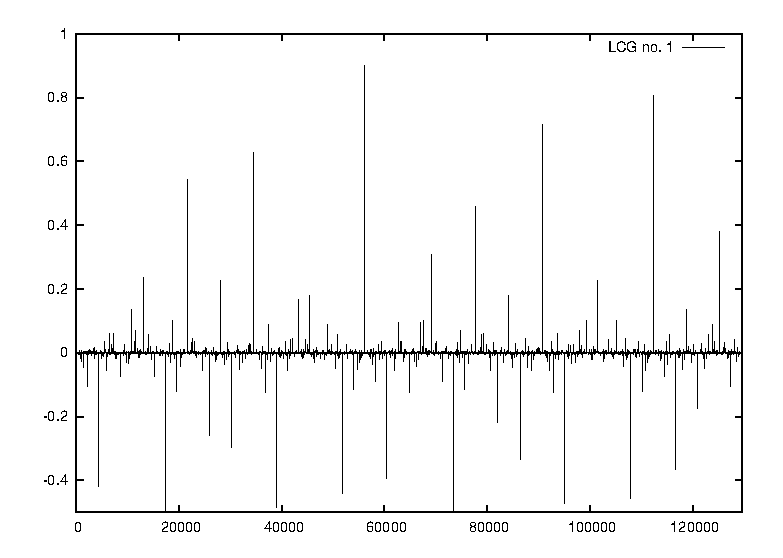
\includegraphics{ranfst10_lcg1.eps}}}\quad
\subfloat[Sequence no.2]
{\resizebox{!}{35mm}{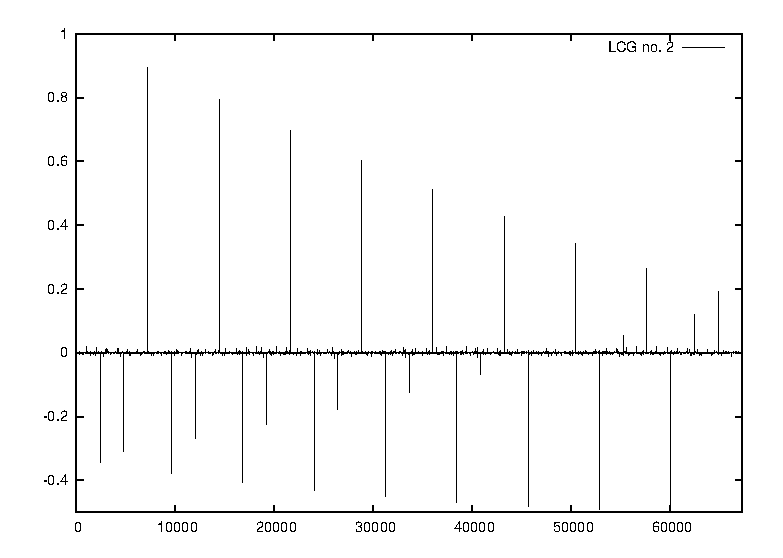
\includegraphics{ranfst10_lcg2.eps}}}\quad
\subfloat[Sequence no.3]
{\resizebox{!}{35mm}{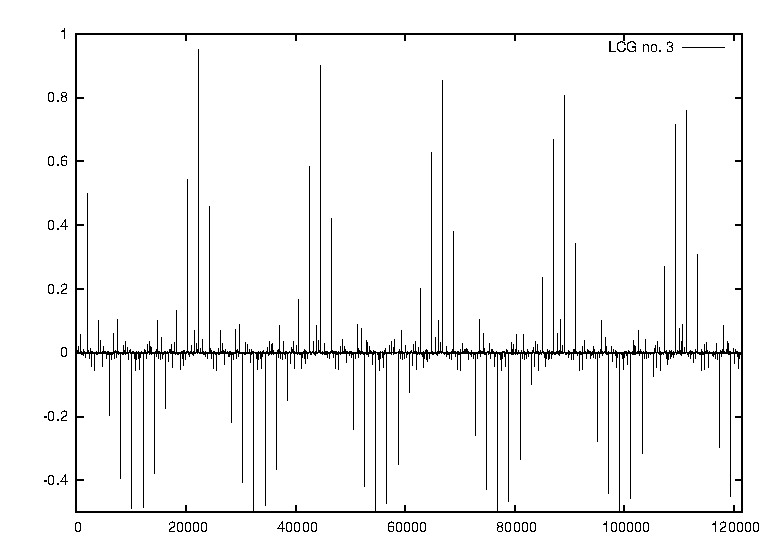
\includegraphics{ranfst10_lcg3.eps}}}\quad
\subfloat[Sequence no.4]
{\resizebox{!}{35mm}{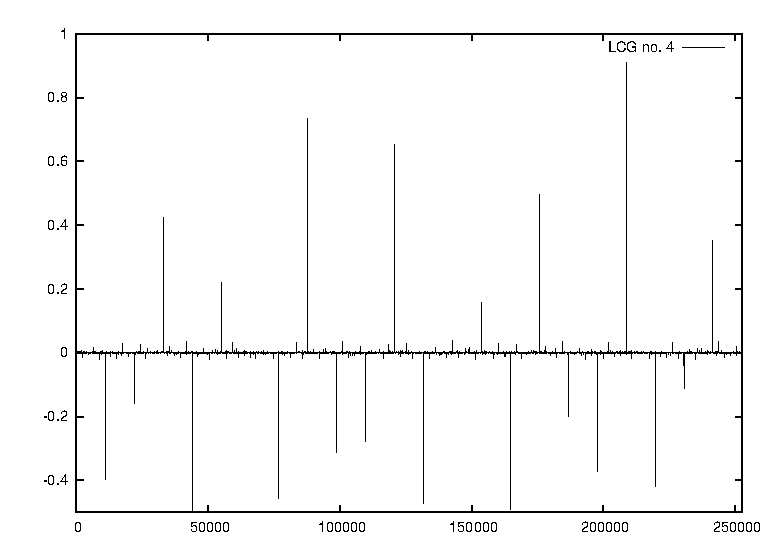
\includegraphics{ranfst10_lcg4.eps}}}\quad
\subfloat[Sequence no.5]
{\resizebox{!}{35mm}{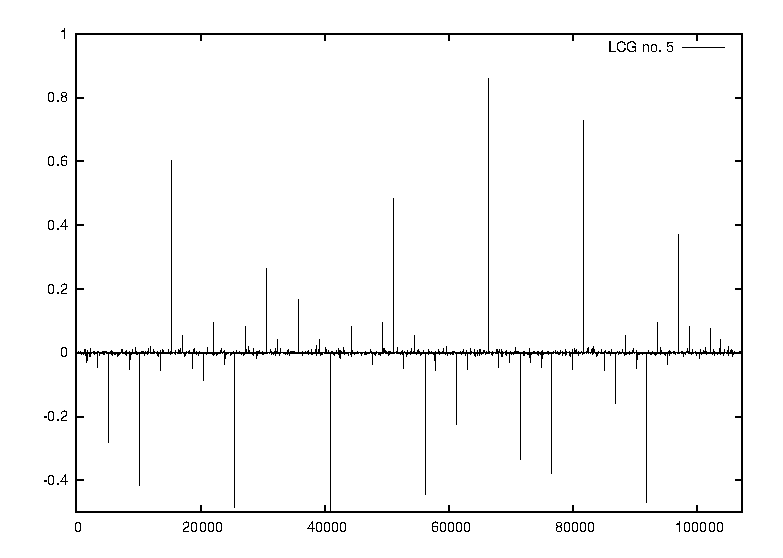
\includegraphics{ranfst10_lcg5.eps}}}\quad
\subfloat[Sequence no.6]
{\resizebox{!}{35mm}{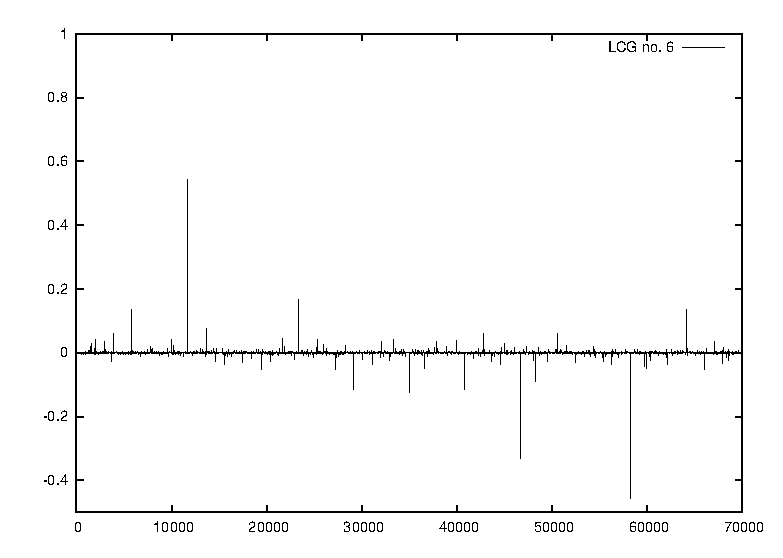
\includegraphics{ranfst10_lcg6.eps}}}\quad
\subfloat[Sequence no.7]
{\resizebox{!}{35mm}{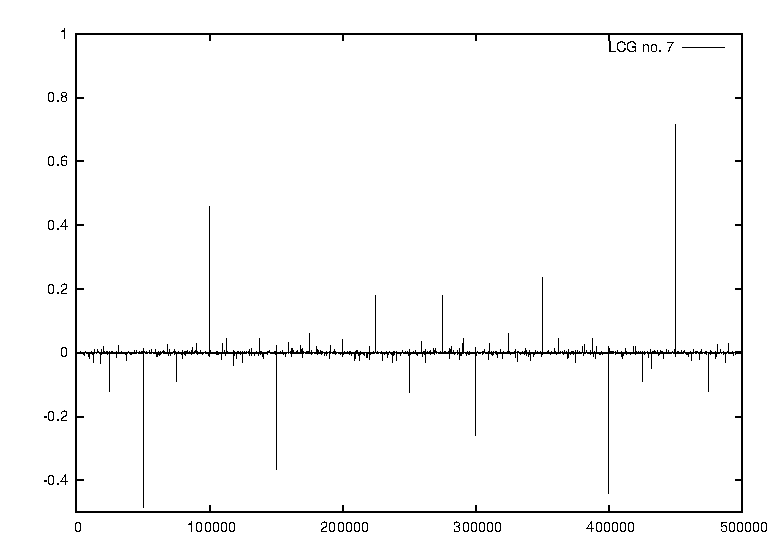
\includegraphics{ranfst10_lcg7.eps}}}\quad
\label{figautolcg}
\caption{Autocorrelation functions for linear congruential sequences}
\end{center}
\end{figure}
Clearly none of the sequences is free from some degree of correlation,
as revealed by the occurrence of isolated sharp spikes in the
autocorrelation function.  For sequences having even period length $m$ there is a spike
of magnitude $-1/2$ at a lag of $m/2$ - it can be shown \cite{knuth} using the
expression (\ref{recurgen}) that this is an
intrinsic property of the linear congruential method.  The
cross--correlation function $c^{Y(1,2)}_{i}$ was evaluated for each
linear congruential sequence by changing the starting value $Y^{(2)}_{1}$
- as expected this simply shifts the pattern observed in the
autocorrelation function, by an amount that depends on the location
of the starting value within the sequence.

Autocorrelation functions were also evaluated for the combined and shuffled
sequences, and results are shown in Figure \ref{figautocombo}.
\begin{figure}[htbp]
\begin{center}
\subfloat[Combined sequence no.1]
{\resizebox{!}{50mm}{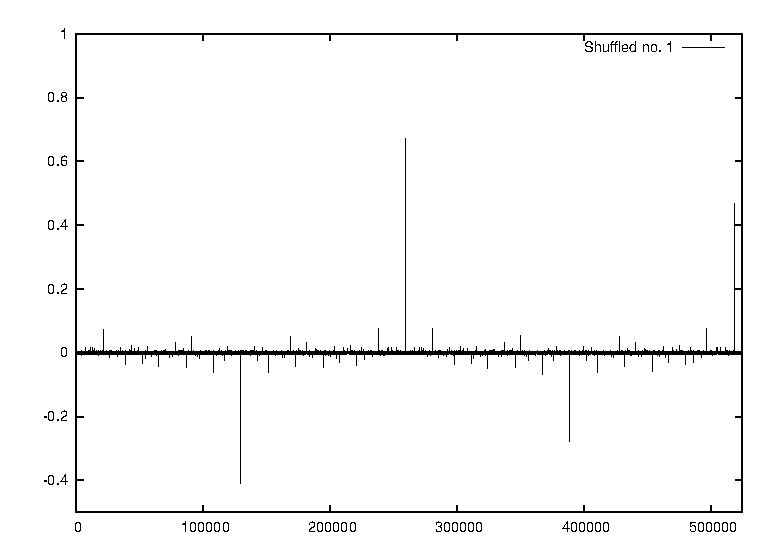
\includegraphics{ranfst10_shuff1.eps}}}\quad
\subfloat[Combined sequence no.2]
{\resizebox{!}{50mm}{\includegraphics{ranfst10_shuff2.eps}}}\quad
\caption{Autocorrelation functions for the combined and shuffled sequences}
\label{figautocombo}
\end{center}
\end{figure}
Here it is not feasible to use the full period of the sequence and a sample of
length 1048576 was used for sequence no.1, and 2097152 for sequence
no.2.  For sequence no.1 there is evidence of non--zero correlation at the
period length of the
linear congruential sequence used to generate the low--order segment, but
the magnitude of the correlation spikes has been reduced by the shuffling
algorithm.  Sequence no.2 appears to be essentially free of significant
correlation, even over the much longer sample size tested.  Tests on the
length of the shuffling array with values up to 997 revealed very little
sensitivity to this parameter.  Cross--correlation of the combined and shuffled
sequence with different starting values showed very low values throughout.

Finally the combined and shuffled sequences were sub--sampled by taking
every third element, starting in turn with elements 1, 2 and 3.  This
reflects the manner in which the sequence is likely to be used for
initialisation of a DNS.
Autocorrelation of each sub--sampled sequence showed similar behaviour to
that of the full sequence, while cross--correlation again returned very
low values.
 
\subsection*{Conclusions}
Investigation of the properties of random number generators suitable for
use in DNS of turbulent flow has been carried out using theoretical,
statistical and correlation techniques.  An overriding requirement is
that the random number generator routine should be portable, and
therefore must be written in a standard high level language.  This
places a restriction on the maximum integer value that can be
represented.  Linear
congruential sequences are computationally efficient and may be designed
to have well--defined properties, but testing remains essential.  Such
sequences are periodic on lengths which are too short for present
purposes, and also exhibit regular correlations on fractions of the period
length.  Two linear congruential sequences may be combined to yield a
sequence having very much greater period length, and a simple shuffling
algorithm may be used to smear out unwanted correlations and further to
extend the period length to values well beyond those of present concern.
Such combined and shuffled random number generators have adequate
equidistribution properties across the interval of interest, and are
reasonably free of correlations that could contaminate an initial
turbulent field.  In particular, there is no appreciable correlation
between subsequences consisting of every third element of the main
sequence: this ensures that the angles required at each point are
uncorrelated.  Similarly, there is no appreciable correlation between
sequences generated using different starting values: this ensures that
initial turbulent fields generated by separate processors of a parallel
computer will remain uncorrelated provided that a different seed is used
to initialise the random number generator on each processor.

\newpage
\begin{thebibliography}{99}
\bibitem{orszaginit}S.A. Orszag: Numerical methods for the simulation of
turbulence, Phys. Fluids Suppl. II, 250--257, 1972.
\bibitem{rogallo}R.S. Rogallo: Numerical experiments in homogeneous
turbulence, NASA Tech. Memo. 81315, 1981.
\bibitem{leereynolds}M.J. Lee, W.C. Reynolds: Numerical experiments on
the structure of homogeneous turbulence, Technical Report TF--24,
Thermosciences Division, Dept. of Mechanical Engineering, Stanford University,
1985.
\bibitem{batchelor53}G.K. Batchelor: {\it The Theory of Homogeneous
Turbulence}, Cambridge University Press, 1953.
\bibitem{schupatt}U. Schumann, G.S. Patterson: Numerical study of pressure
and velocity fluctuations in nearly isotropic turbulence, J. Fluid Mech.
{\bf 88}, 4, 685--709, 1978.
\bibitem{batchelortownsend}G.K. Batchelor, A.A. Townsend: Decay of
turbulence in the final period, Proc. Roy. Soc. Lond. {\bf A194}, 527--543,
1948.
\bibitem{moninyag}A.S. Monin and A.M. Yaglom: {\it Statistical Fluid
Mechanics}, Vol.1, Mechanics of Turbulence, ed. J.L. Lumley, MIT
Press, 1971.
\bibitem{temperton}C. Temperton: A generalised prime factor FFT
algorithm for any $N=2^{p}3^{q}5^{r}$, SIAM J. Sci. Stat. Comp. {\bf 13},
676--686, 1992.
\bibitem{roballan}R.J. Allan:  Parallel application software on high
performance computers: serial and parallel FFT routines, CSED Report,
Daresbury Laboratory, UK, ISSN 1362--0193, 2nd ed., 1999.
\bibitem{hinze}J.O. Hinze: {\it Turbulence}, McGraw--Hill, 2nd ed., 1975.
\bibitem{eisele+mason}J.A. Eisele, R.M. Mason: {\it Applied Matrix and Tensor
Analysis}, John Wiley and Sons, 1970.
\bibitem{knuth}D.E. Knuth: {\it The Art of Computer Programming}, Vol.2,
Seminumerical Algorithms, Addison--Wesley, 1969.
\bibitem{numrec}W.H. Press, S.A. Teukolsky, W.T. Vetterling, B.P. Flannery:
{\it Numerical Recipes}, Cambridge University Press, 3rd ed., 2007.
\end{thebibliography}

\end{document}
